\chapter{Varying Methods and Parameters}\label{ch:lex}\label{ch:cat}\label{ch:interaction}\label{ch:feedback}\label{ch:par}

The previous chapter extensively presented the basic experiment. The results were not very satisfying, although closer investigation revealed not so bad results. In this chapter, variants of the basic experiment are investigated and compared with this experiment.

What is the impact on categorisation and lexicon formation when a different categorisation mechanisms is used? What influence has the physical conditions on the symbol grounding? What is the impact from applying joint attention and/or feedback? How do various parameter settings of the word-form creation probability and learning rate influence the experiments? And, what if the robots also adopt word-forms when there is a mismatch in referent? These questions will be addressed in this chapter.

To answer these questions, a set of experiments have been carried out. Each experiment is done with 10 runs of 5,000 language games, as in the basic experiment. Unless otherwise mentioned, the basic data set is used in these experiments. Each section of this chapter relates to one of the questions and it presents some of the experiments. The sections introduce the problem addressed. They describe the difference(s) of the experiments, usually in relation to the basic experiment. Then the experimental results are given, which is followed by a short discussion of these results.


The next section investigates three variants of categorisation in the discrimination games. In \sectref{s:par:int}, the physical conditions are varied. The four different types of language games introduced in \chapref{ch:lg}, the guessing, ostensive, observational and XSL game, will be investigated in \sectref{s:par:feed}. Section \ref{s:par:observ} investigates the observational game in more detail. In \sectref{s:par:ps} the creation probability is varied. The learning rate is varied in \sectref{s:par:lr}. Additional word-form adoption is investigated in \sectref{s:par:adopt}. The chapter finishes with a summary.

\section{Impact From Categorisation}\label{s:par:cat}
\index{categorisation|(}
\index{category|(}

In the basic experiment the categories are prototypical as introduced in \sectref{s:cm:prototype}. When a category is used as a meaning that a robot successfully uses in a language game, the value of the category shifts towards the feature value of the relevant sensory channel. What happens if the categories do not shift towards these feature values?

Categorisation is implemented such a that feature vector is always categorised with the prototypes that are closest in each feature space. It has been argued that categorisation is not so clear-cut, but that there may be fuzzy boundaries between adjacent categories (see e.g. \citealt{aitchison:1987} and \citealt{lakoff:1987}). Especially around the boundaries of a category's sensitivity, the certainty of whether a feature vector belongs to one category or another becomes smaller. For instance, something that looks like a {\em cup} might be categorised by another person as a {\em vase} or {\em bowl} as has been shown by \citet{labov:1973}. {\em Family resemblance} \citep{wittgenstein:1958} is another example of such fuzziness.  These are examples at a higher level of categorisation, but the same may hold at the lower level of categorisation.\index{family resemblance}\index{Wittgenstein, Ludwig}

These two questions are investigated in this section, together with the binary subspace method (see \sectref{s:cm:binary}). The results are compared with the basic experiment.

\subsection{The Experiments}

There are the following experiments (all are variants of the basic experiment, and thus implement the guessing game):

\begin{description}
\item[NS] No shifting categories. Once a prototypical category is introduced, its value does not change through time. Hence the categories are static.

\item[FS] Fuzzy sets. Categories may overlap each other at their boundaries. In this experiment, a feature is categorised with those categories that are closer than a certain minimal distance, and if no such category exists, the feature is categorised with the category that is closest to the feature value. \index{category!fuzzy}

More formally, a category $c_k$ can be defined by region in a feature space ${\mathcal F}_\lambda$. The category $c_k$ can be described as $c_k=\langle {\bf c}_k,d_k,\nu_k,\rho_k,\kappa_k \rangle$, where ${\bf c}_k=(x_0,\ldots,x_{n-1}$ is a prototype in the $n$ dimensional feature space ${\mathcal F}_\lambda$, $d_k=\frac{1}{2} \cdot 3^{-\lambda}$ is a distance based on the feature space in which the prototype is stored and $\nu_k, \rho_k \mbox{and} \kappa_k$ are scores as described in \chapref{ch:lg}. The distance $d_k$ is based on an equal subdivision of the number of exploitations that are done in the feature space ${\mathcal F}_\lambda$.

A feature vector is {\bf f} is categorised with $c_k$ if its distance to ${\bf c}_k$ is shortest, or if in each dimension $i$ the distance between $f_i$ and $x_{k,i}$ is smaller than $d_k$, i.e. $|f_i-x_i|<d_k$. 

Note that in this way a feature vector may be categorised with more than one category in each feature space. If the vector is closest to the prototype of one category, but if it falls inside the region of another category as defined by $d_k$, it is categorised in two or more ways. It is also important to realise that, like in the prototype method, whenever there exists a prototype in some feature space ${\mathcal F}_\lambda$, a feature vector can be categorised in this space.

So, instead of one possible categorisation in each feature space, a feature vector may have several. This increases the chance that a referent is categorised more parsimoniously and thus increasing the communicative success. Note that the discrimination game is unaltered.

\item[BIN] Binary subspace method. See \sectref{s:cm:binary}.
\end{description}

\subsection{The Results}

The results compared with the basic experiment are given in \figref{f:par:cat} and \tabref{t:par:cat}. These results give the global averaged results of the communicative success, discriminative success, distinctiveness, parsimony, specificity and consistency.

\begin{figure}
\centering
\subfigure[CS]{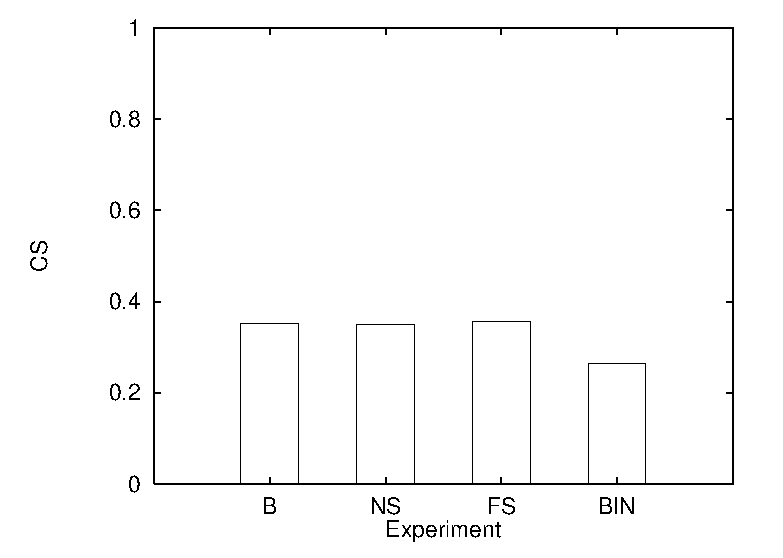
\includegraphics[width=5.5cm]{categorization/rescs.eps}}
\subfigure[DS]{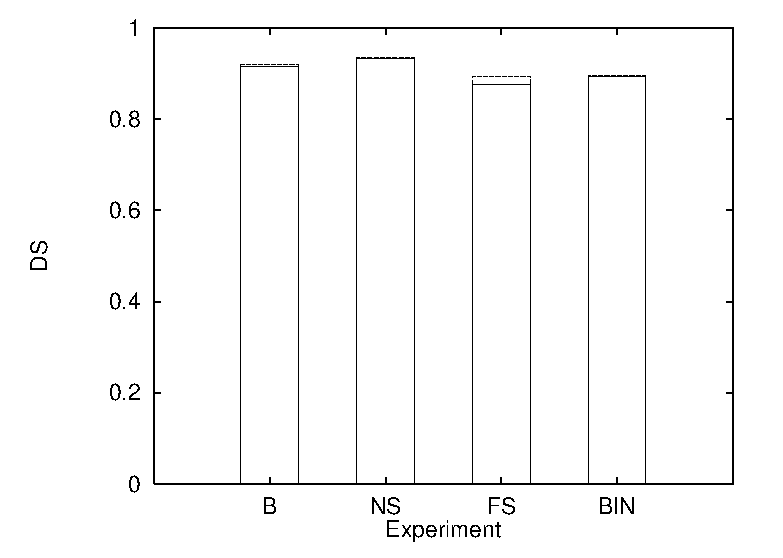
\includegraphics[width=5.5cm]{categorization/resds.eps}}\\
\subfigure[S]{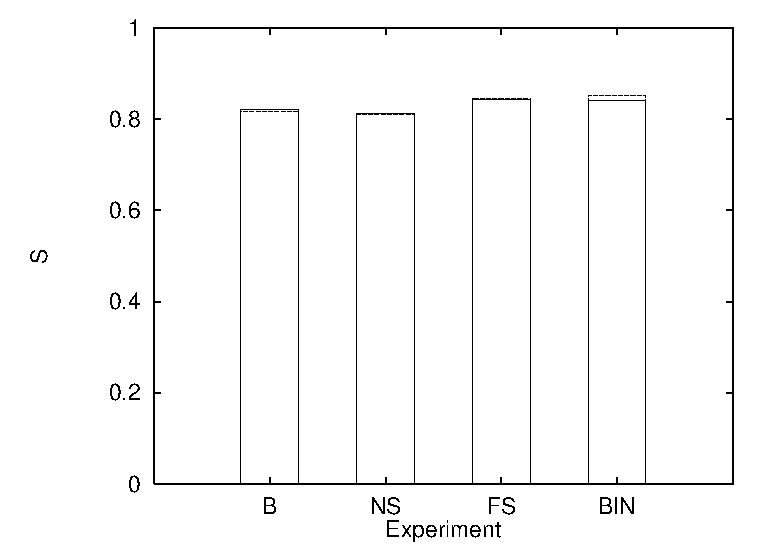
\includegraphics[width=5.5cm]{categorization/resspec.eps}}
\subfigure[D]{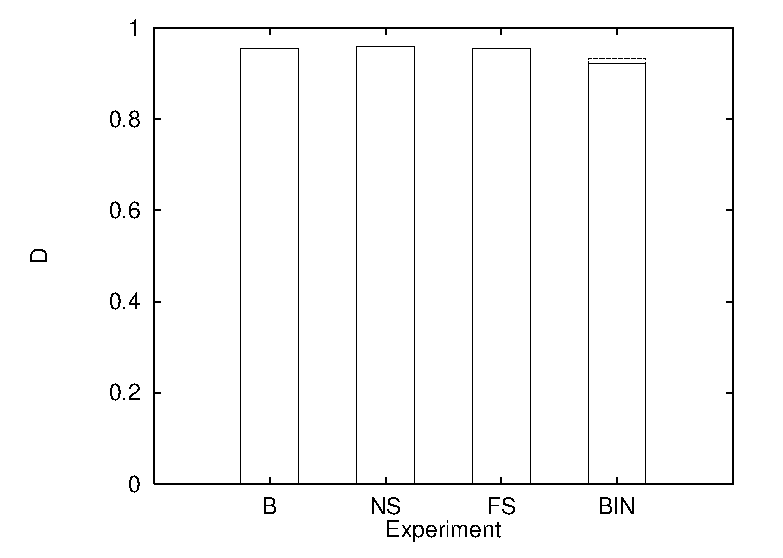
\includegraphics[width=5.5cm]{categorization/resdist.eps}}\\
\subfigure[C]{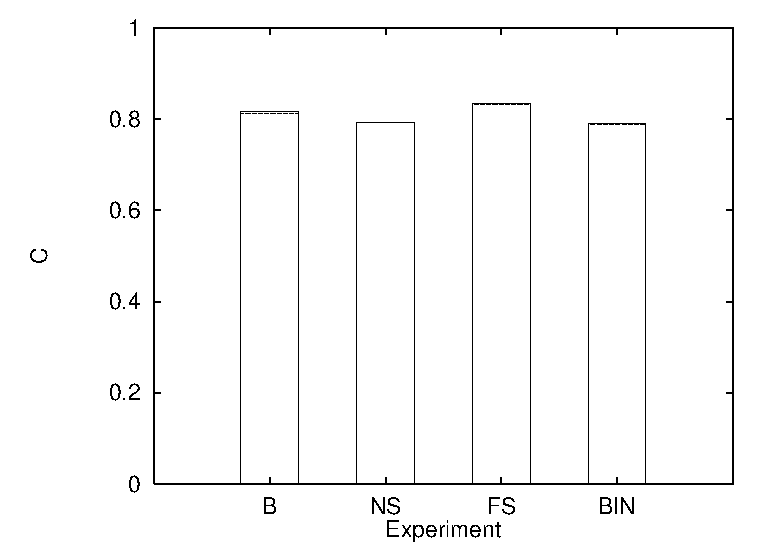
\includegraphics[width=5.5cm]{categorization/rescons.eps}}
\subfigure[P]{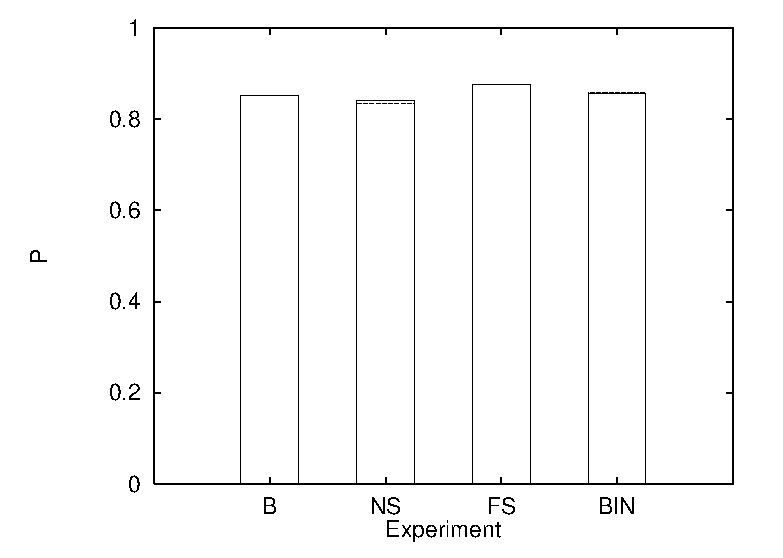
\includegraphics[width=5.5cm]{categorization/respars.eps}}
\caption{The average scores of the experiments discussed in this chapter: static categories (NS), fuzzy sets (FS) and binary subspaces (BIN) compared with the basic experiment (B).}
\label{f:par:cat}
\end{figure}

\begin{table}[t]
\centering
\begin{tabular}{l d{3}@{~}c@{~}d{3} d{3}@{~}c@{~}d{3} d{3}@{~}c@{~}d{3} d{3}@{~}c@{~}d{3}}
\lsptoprule
        & \multicolumn{3}{c}{B}               &   \multicolumn{3}{c}{NS}      &  \multicolumn{3}{c}{FS}             &  \multicolumn{3}{c}{BIN}\\\midrule
CS      & 0.351& $\pm$ & 0.010 &   0.349& $\pm$ & 0.017&  0.357& $\pm$ & 0.024&  0.264& $\pm$ & 0.041\\%\hline
DS0     & 0.916& $\pm$ & 0.004 &   0.933& $\pm$ & 0.007&  0.875& $\pm$ & 0.014&  0.893& $\pm$ & 0.005\\%\hline
DS1     & 0.920& $\pm$ & 0.004 &   0.935& $\pm$ & 0.006&  0.894& $\pm$ & 0.013&  0.895& $\pm$ & 0.003\\%\hline
D0      & 0.956& $\pm$ & 0.002 &   0.959& $\pm$ & 0.000&  0.956& $\pm$ & 0.001&  0.922& $\pm$ & 0.005\\%\hline
D1      & 0.955& $\pm$ & 0.002 &   0.959& $\pm$ & 0.000&  0.956& $\pm$ & 0.001&  0.933& $\pm$ & 0.003\\%\hline
P0      & 0.852& $\pm$ & 0.004 &   0.841& $\pm$ & 0.005&  0.875& $\pm$ & 0.003&  0.856& $\pm$ & 0.004\\%\hline
P1      & 0.851& $\pm$ & 0.002 &   0.835& $\pm$ & 0.006&  0.875& $\pm$ & 0.002&  0.858& $\pm$ & 0.007\\%\hline
S0      & 0.822& $\pm$ & 0.017 &   0.813& $\pm$ & 0.022&  0.843& $\pm$ & 0.022&  0.841& $\pm$ & 0.045\\%\hline
S1      & 0.817& $\pm$ & 0.011 &   0.810& $\pm$ & 0.015&  0.846& $\pm$ & 0.024&  0.852& $\pm$ & 0.040\\%\hline
C0      & 0.816& $\pm$ & 0.008 &   0.793& $\pm$ & 0.007&  0.835& $\pm$ & 0.011&  0.791& $\pm$ & 0.016\\%\hline
C1      & 0.811& $\pm$ & 0.007 &   0.793& $\pm$ & 0.007&  0.832& $\pm$ & 0.008&  0.789& $\pm$ & 0.023\\%\hline
\lspbottomrule
\end{tabular}
\caption{The results of the experiments on categorisations. The columns give the averaged results with their standard deviation of the basic experiment (B) compared with experiments NS, FS and BIN.}
\label{t:par:cat}
\end{table}

\begin{description}
\item[NS] Experiment NS shows that there are hardly any {\em significant} differences compared to the basic experiment. The discriminative success is about 1.5 \% higher with a significance of $p=0.0052$. The parsimony and consistency appears to be lower with a $p$-value of resp. $p=0.0432$ and $p=0.0354$. All other differences have no significance at all. So, although one might expect larger differences they have not been observed. If there is a function for shifting the categories it will be for increasing parsimony and consistency, but this has not been observed with much certainty.
\index{category!static}

\item[FS] The results of the FS experiments show that although there are more possible meanings, the discriminative success is lower than in the basic experiment ($p=0.0000$). The communicative success shows an insignificance difference ($p=0.1230$). However,  one run showed an exceptional small communicative success, namely 0.23. When throwing away this run (which is statistically valid) the average communicative success becomes $0.371 \pm 0.025$ which is different with a $p$-value of $p=0.0504$. So, although this looks better, it is hard to say whether the communicative success of this experiment is better. 

The distinctiveness is equal to the basic experiment. The specificity seems to be higher than in the basic experiment and the consistency seems to be lower, but these differences are insignificant ($p=0.2176$ and $p=0.1230$ resp.). The parsimony however is slightly higher (0.02) with a significance of $p=0.0008$.

So, although the discriminative success is lower than in the basic experiment, the fuzzy set approach does not appear to influence the quality of the communication system that emerges. \index{category!fuzzy}

\item[BIN] When examining the BIN experiment, a first thing that strikes is the lower discriminative success ($p=0.0004$). This lower discriminative success is because it increases slower (\figref{f:cat:bin} b). It finally increases to the same level as in the basic experiment (see \figref{f:st:plot} at page \pageref{f:st:plot}).

\index{binary!subspace method}
The communicative success stays well behind the communicative success of the basic experiment ($p=0.0016$). It is not directly clear why the communicative success is about 8.5 \% lower. The communicative success appears to stop learning after 1,000 language games, although it seems to increase slowly again after 4,000 games (\figref{f:cat:bin} a). The consistency is about 0.025 lower than in the basic experiment ($p=0.0354$), but parsimony is $\pm 0.005$ higher ($p=0.0524$). Because the $p$-values are relatively high, it is difficult to assign meaning to these differences.

Most significant difference is the distinctiveness, which is $\pm 0.03$ lower with a significance of $p=0.0002$. In contrast to previous plots that have been shown the distinctiveness does not grow towards a value of 1, but it stabilises around 0.97 (\figref{f:cat:bin} c). So, it seems that the meanings less reliably refer to the corresponding referents, thus indicating more one-to-many relations between a meaning and the referents. Specificity is higher than in the basic experiment indicating that polysemy is less. This observation, however, has a low significance: $p=0.1904$. Hence lower distinctiveness might explain a lower communicative success, since a word-meaning no longer refers to one referent, which it does when $D=1$.
\end{description}

\begin{figure}[t]
\centering
\subfigure[CS]{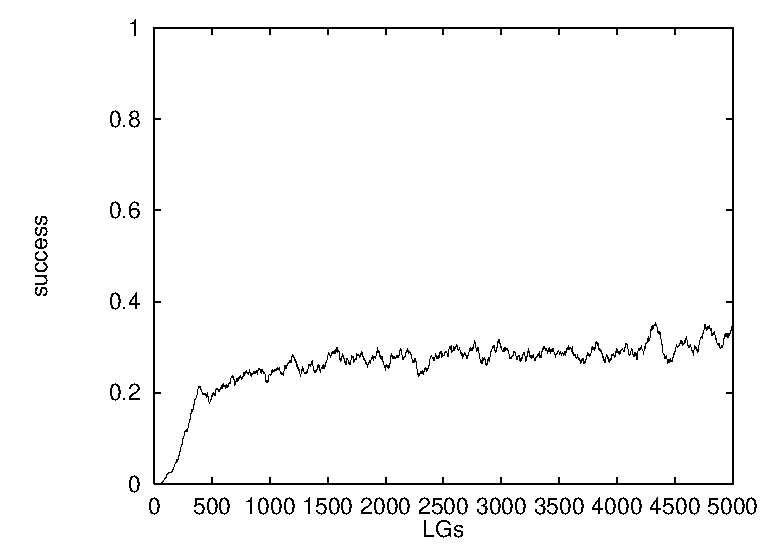
\includegraphics[width=5.5cm]{categorization/csbin.eps}}
\subfigure[DS]{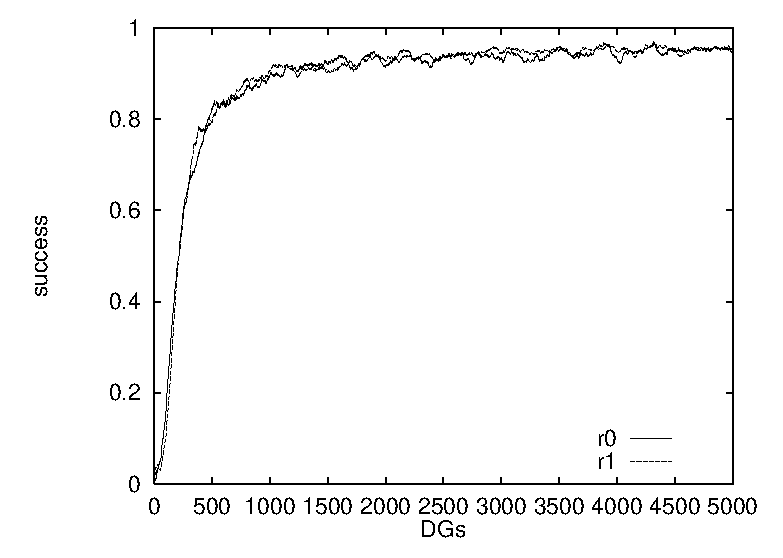
\includegraphics[width=5.5cm]{categorization/dsbin.eps}}\\
\subfigure[D]{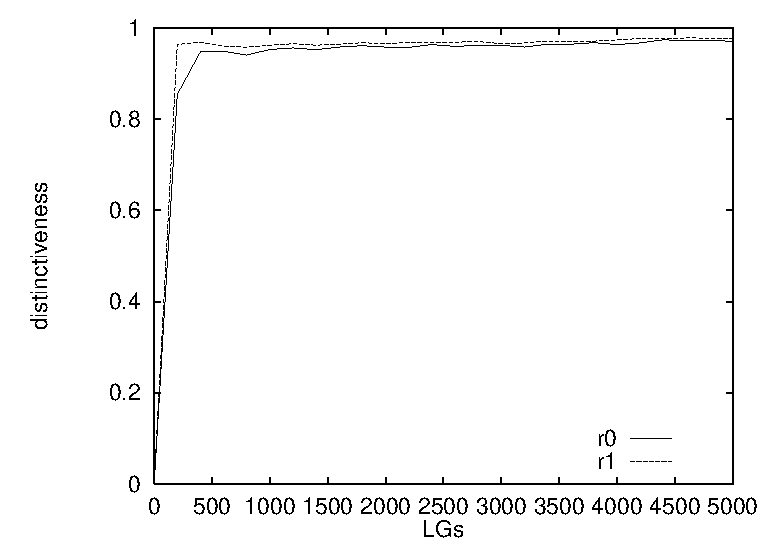
\includegraphics[width=5.5cm]{categorization/dbin.eps}}\\
\caption{The evolution of the some measures for the binary subspace method.}
\label{f:cat:bin}
\end{figure}

\subsection{Discussion}

When the prototypes do not shift towards the central tendency as is the case in experiment NS, the communication system that is developed is qualitatively about the same. So, in the current set up, the dynamics of categories does not add any other functionality than possibly a more realistic model.


There is psychological and linguistic evidence that categories overlap making way for a fuzzy approach to categorisation. An experiment has been done where categories can overlap near their edges (or even near their centre when they are very close to each other). The discriminative success is significantly worse than in the basic experiment and the communicative success improves slightly but this is not very significant. It was predicted that parsimony and consistency would improve since the robots get a better chance to choose meanings or word-forms more consistently. This however, has only been observed for the parsimony; the difference in consistency was insignificant.


The binary subspace method is performing worse than the basic set-up, which is a bit surprising. The communicative success is lower than chance and the discriminative success is lower than originally. The latter observation has much to do with a slow start. In the prototype method if an agent has constructed a category at a particular feature space, the agent can categorise every segment at this layer and sensory channel. This is because a feature is categorised with the category that is {\em closest} to the feature value. In the binary subspace method, this is not the case because each category has a fixed size and a feature space ${\mathcal F}_\lambda$ needs not to be covered completely with categories. Since a feature value must be {\em within} the sensitivity of an existing category, a segment may not always be categorised. At a later stage, the feature spaces are covered to a higher degree, so the discriminative success increases towards the end.

The system's distinctiveness is significantly different, but for the other measures parsimony, specificity and consistency the differences are much less significant or maybe not at all. So, in the binary subspace method more one-to-many relations between referent and meaning emerge than in the prototype method.
\index{category|)}
\index{categorisation|)}

\section{Impact From Physical Conditions and Interactions}\label{s:par:int}


In the basic experiment, the robots decided to stop after two rotations based on finding a maximum intensity of infrared on the left back infrared sensor. Another method described is letting the robots align each other using infrared taxis (\sectref{s:robots:PDL}). Besides longer experimental time (due to more error-prone physical behaviour) the taxis has no influence on the grounding process, since the taxis is applied {\em after} the sensing. Two experiments are done where taxis is used to align the robots. In the first experiment it was observed that the gearing of the robots were worn off. In the second experiment the gearing were replaced by new ones. These experiments show how co-ordination abilities and physical fitness may influence the quality of interactions.

In \citealt{steelsvogt:1997} the robots did not rotate twice aligning back-to-back while doing the sensing, but only once aligning face-to-face. This experiment has been repeated to see what the differences are.

The adaptation of an agent to its environment and the agent's ability to detect the environment with enough precision is likely to be very important. In one experiment the environment and robots are changed such that the resolution of the robots' sensing decreases.

In all the experiments so far there were constantly 4 light sources present in the robots' environment. What happens when in each situation there are only 3 light sources present, while the robots' niche has 4 light sources? The last experiment of this section investigates this.

\subsection{The Experiments}

The experiments of this section all investigate the impact from physical interactions and -conditions on the robots' ability to ground a lexicon. Again all the experiments are variants of the basic experiment and hence implement the guessing game. The following experiments are defined:

\begin{description}
\item[WOG] Worn-off gearing. In this experiment the gearing of the robots were completely worn-off. As a result the robots had difficulties in rotating during the sensing task. Taxis is applied to re-align the robots after sensing.

\item[NG] New Gearing. The robots in this experiment are equipped with brand new gearing. Like in WOG, taxis is applied to re-align the robots. \index{gearing}

\item[A] Acceleration. In the original implementation the robots rotate only once starting face-to-face \citep{steelsvogt:1997} rather than rotating twice and starting back-to-back. When the robots rotate once they immediately start the sensing and first have to accelerate, thus the spatial view initially is somewhat warped. When rotating twice they start sensing when the rotating robot faces its opponent. This way the robot is already moving at a constant speed, whereas in the original implementation the robots first have to accelerate.

\item[RD] Reducing distinctiveness. In this experiment the difference in heights were reduced to 1.9 cm instead of 3.9cm. This way the environment is reduced. Figure \ref{f:int:calibration} shows the characteristics of the sensors as measured for different distances when facing a light source. It is obvious that the further a robot gets away from the light source, the closer the different sensor readings are. Furthermore, it should be clear that when the distance between robot and light source is larger, correspondence between sensor and light source is unreliable. Hence, the feedback mechanism is unreliable. Interesting to see is that when the robot is close to the light source the non-corresponding sensors hardly sense light, but up to 40 cm the intensities increase. This is because at close distance the light source is invisible for these sensors and at larger distance the divergent light emission falls on the sensors. Naturally it is expected that the robots have more difficulty in discriminating and identifying the light sources.\index{sensors light}

\item[DE] Dynamic environment. In this experiment there were only three light sources present in every recorded situation. The height of the light sources were the same as in the basic experiment. After every few games, one of the light sources was removed and the one that was already out of the environment has been placed back. Whereas in the other experiments all light sources stayed roughly at the same place, the position of the light sources changed in this experiment as well. This way a dynamic environment was created.
\end{description}


\begin{figure}[t]
\centering
\subfigure[L0]{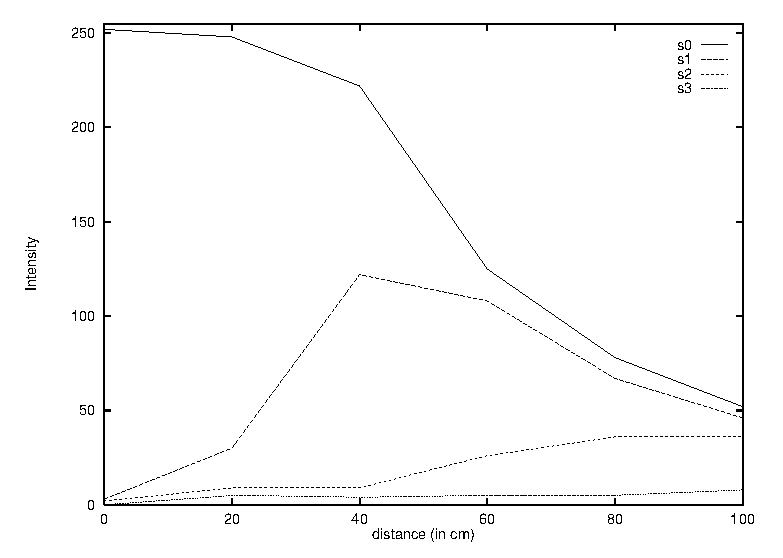
\includegraphics[width=5.5cm]{physical/sensors0.eps}}
\subfigure[L1]{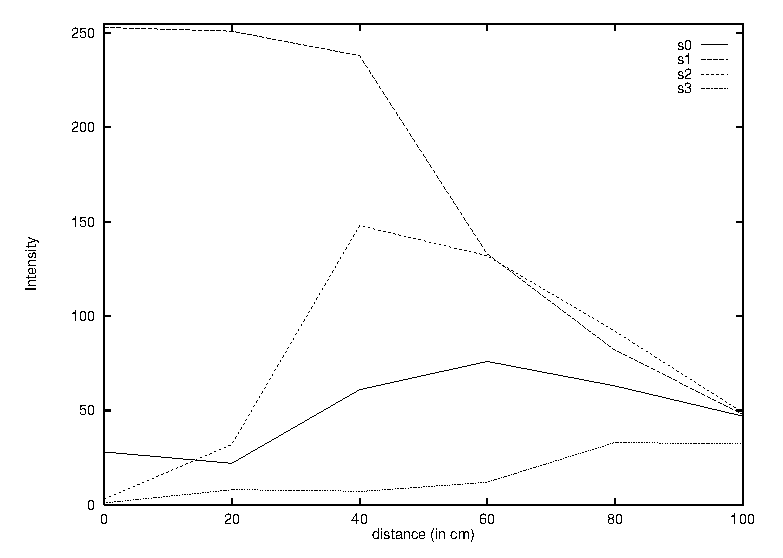
\includegraphics[width=5.5cm]{physical/sensors1.eps}}\\
\subfigure[L2]{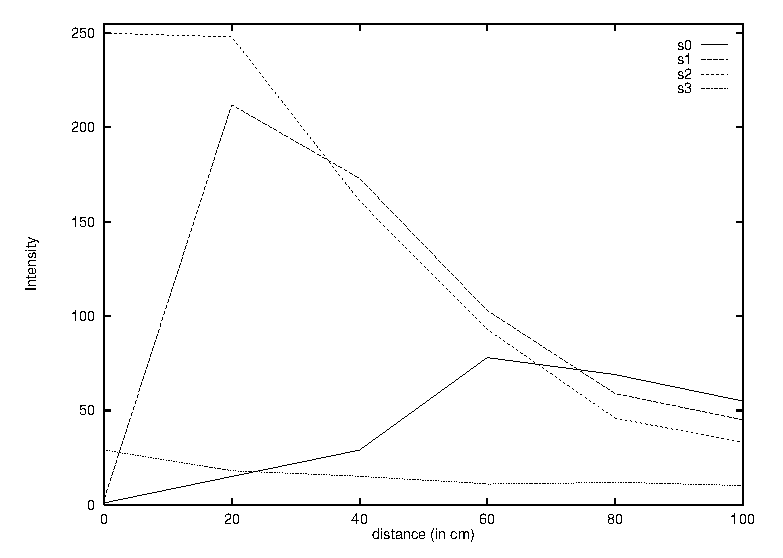
\includegraphics[width=5.5cm]{physical/sensors2.eps}}
\subfigure[L3]{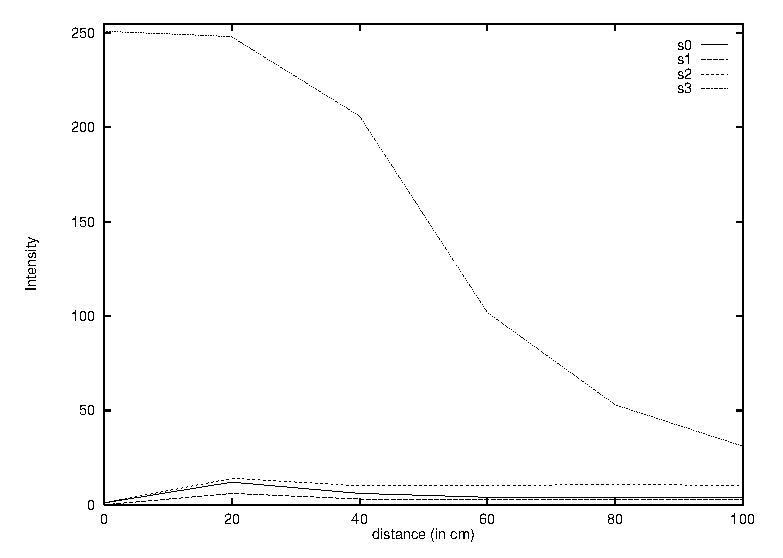
\includegraphics[width=5.5cm]{physical/sensors3.eps}}
\caption{The characteristics of sensors s0, s1, s2 and s3 of robot r0 while looking at light sources (a) L0, (b) L1, (c) L2 and (d) L3. The light sources are placed at heights with a difference of 1.9 cm in between. Note that the characteristics of L3 may be inaccurate since the characteristics is quite different from all other characteristics.}
\label{f:int:calibration}
\end{figure}

\subsection{The Results}

For all the experiments, different sensory data had to be recorded. Investigating the sensory data revealed the statistics given in \tabref{t:par:stats}.

\begin{table}
\centering
\begin{tabular}{lr@{~}d{2}d{2}d{1}d{1}d{1}}
\lsptoprule
Exp & \#Sit & \multicolumn{1}{c}{$\langle | Cxt | \rangle_{r0}$} & \multicolumn{1}{c}{$\langle | Cxt | \rangle_{r1}$} & \multicolumn{1}{c}{APS (\%)} & \multicolumn{1}{c}{$U_{r0}$ (\%)} & \multicolumn{1}{c}{$U_{r1}$ (\%)}\\\midrule
B & 1017 & 3.33 & 3.54 & 29.1 & 81.1 & 78.0\\%\hline
WOG & 606 & 3.64 & 3.83 & 26.8 & 89.7 & 82.4\\%\hline
NG & 934 & 3.28 & 3.49 & 29.6 & 80.9 & 77.9\\%\hline
A & 1360 & 3.55 & 3.35 & 29.0 & 72.2 & 76.4\\%\hline
RD & 953 & 3.53 & 3.48 & 28.5 & 63.9 & 67.9\\%\hline
DE & 980 & 2.86 & 2.90 & 34.7 & 75.7 & 73.8\\%\hline
\lspbottomrule
\end{tabular}
\caption{The statistics of the sensory data of the experiments investigating the physical interactions and conditions. The columns display the experiments (Exp), the number of situations recorded (\#Sit), the context size of robots r0 and r1 ($\langle | Cxt | \rangle_{r}$), the a priori success (APS) and the potential understandability of the two robots ($U_{r}$). The basic experiment (B) is added for comparison.}
\label{t:par:stats}
\end{table}


Looking at this table, one can already see some interesting results. The WOG experiment reveals highest potential understandability. It also has a context size closer to 4 than in the other experiments. Apparently, the robots detect the four referents better when they rotate slower. 

The NG experiment reveals data similar to the basic experiment. This is not surprising, since the only methodological difference with the basic experiment is taxis, which should not influence the grounding. Moreover, the basic experiment is recorded immediately after this experiment, so the physical condition of the gearing were similar.\index{data set!gearing}

Experiment A has lower understandability. Apparently the warping during acceleration has some influence.

RD has most influence on the data. Although the context size is similar (and thus the a priori success), the potential understandability is much lower. It seems there is more confusion.

Making the environment dynamic (DE) has a logical consequence that the context size is almost 3, making the a priori success $\pm 35$\%. The understandability is lower than in the basic experiment.


So, how does the ontology and lexicon evolve in these experiments? The results are shown in \figref{f:par:int} and \tabref{t:par:int}.

\begin{figure}
\centering
\subfigure[CS]{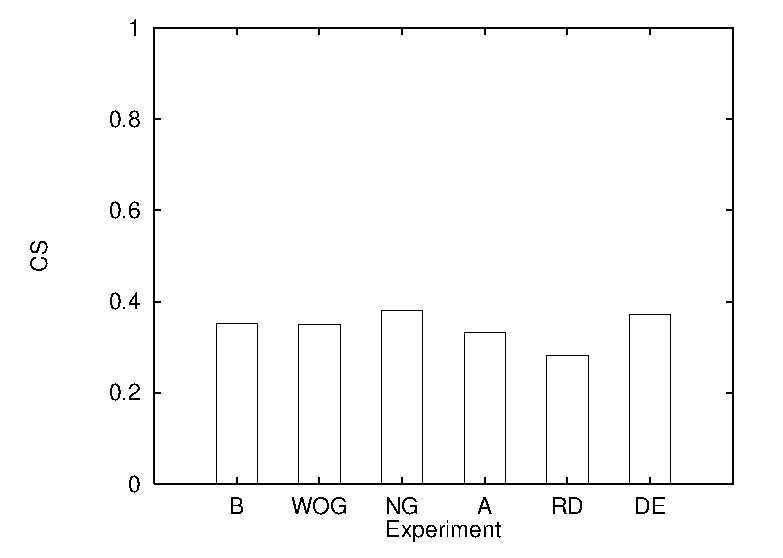
\includegraphics[width=5.5cm]{physical/cs.eps}}
\subfigure[DS]{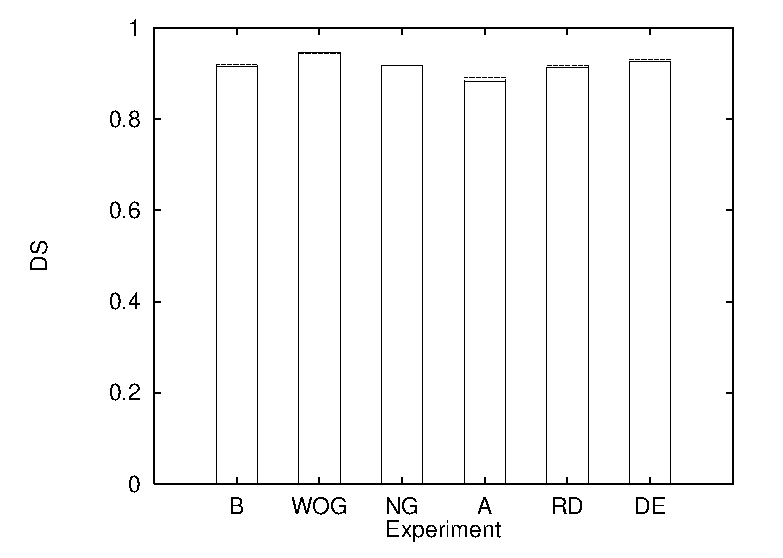
\includegraphics[width=5.5cm]{physical/ds.eps}}\\
\subfigure[S]{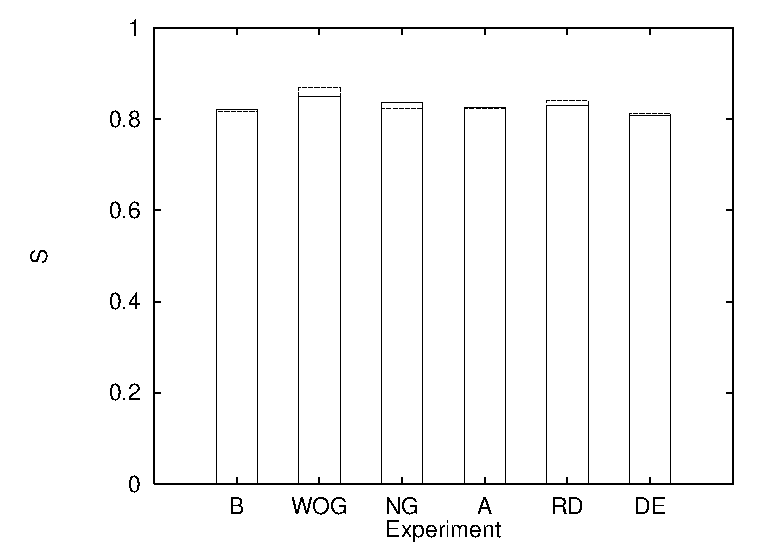
\includegraphics[width=5.5cm]{physical/s.eps}}
\subfigure[D]{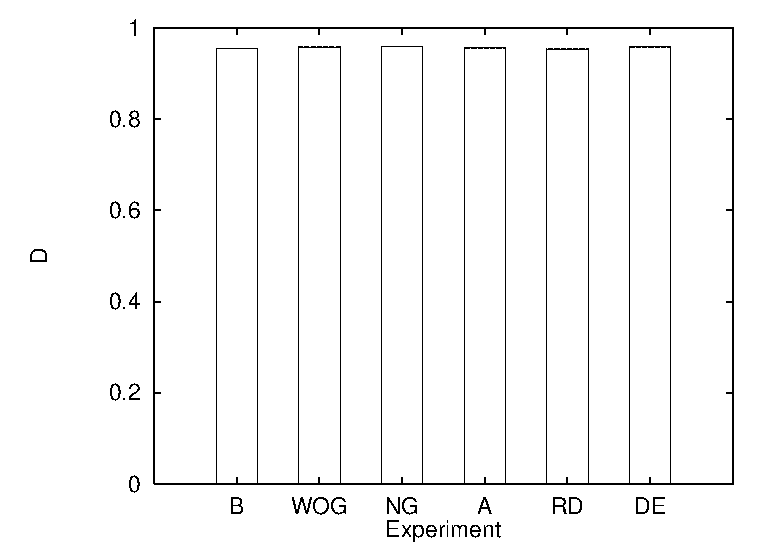
\includegraphics[width=5.5cm]{physical/d.eps}}\\
\subfigure[C]{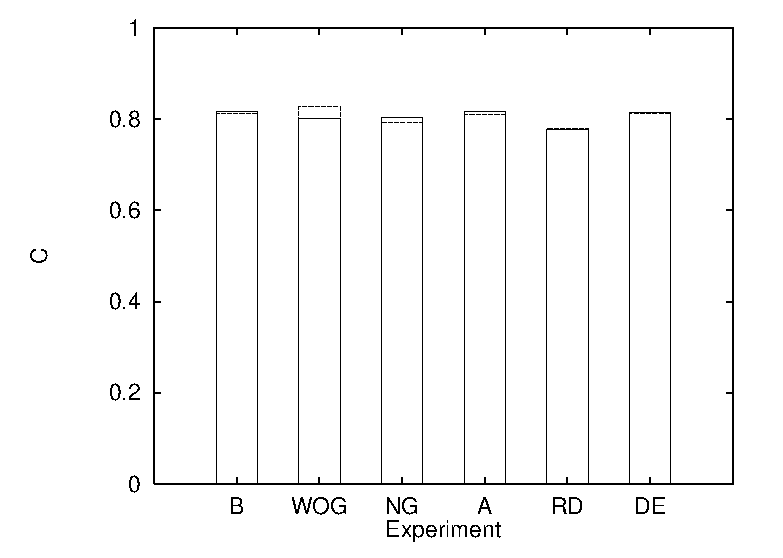
\includegraphics[width=5.5cm]{physical/c.eps}}
\subfigure[P]{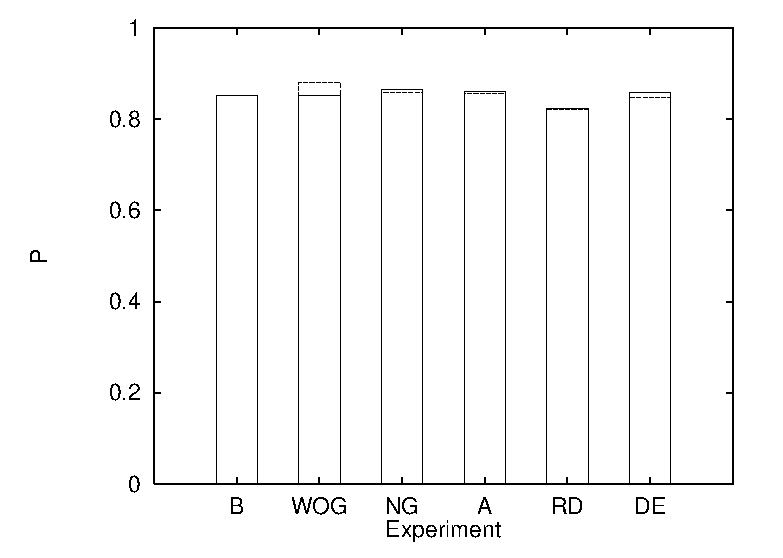
\includegraphics[width=5.5cm]{physical/p.eps}}
\caption{An overview of the results of the experiments presented in this section. Experiments WOG, NG, A, RD and DE are compared with the basic experiment (B).}
\label{f:par:int}
\end{figure}

\begin{table}
\centering
\begin{tabular}{l d{3}@{~}c@{~}d{2} d{3}@{~}c@{~}d{2} d{3}@{~}c@{~}d{3}}
\lsptoprule
         & \multicolumn{3}{c}{B} & \multicolumn{3}{c}{WOG} & \multicolumn{3}{c}{NG}\\\midrule
CS       &0.351 & $\pm$ & 0.01&0.350 & $\pm$ & 0.00&0.379 & $\pm$ & 0.013\\%\hline
DS0      &0.916 & $\pm$ & 0.00&0.945 & $\pm$ & 0.00&0.918 & $\pm$ & 0.003\\%\hline
DS1      &0.920 & $\pm$ & 0.00&0.944 & $\pm$ & 0.00&0.917 & $\pm$ & 0.003\\%\hline
D0       &0.956 & $\pm$ & 0.00&0.956 & $\pm$ & 0.00&0.959 & $\pm$ & 0.000\\%\hline
D1       &0.955 & $\pm$ & 0.00&0.960 & $\pm$ & 0.00&0.960 & $\pm$ & 0.001\\%\hline
P0       &0.852 & $\pm$ & 0.00&0.852 & $\pm$ & 0.00&0.864 & $\pm$ & 0.001\\%\hline
P1       &0.851 & $\pm$ & 0.00&0.880 & $\pm$ & 0.00&0.858 & $\pm$ & 0.002\\%\hline
S0       &0.822 & $\pm$ & 0.01&0.849 & $\pm$ & 0.00&0.837 & $\pm$ & 0.014\\%\hline
S1       &0.817 & $\pm$ & 0.01&0.869 & $\pm$ & 0.01&0.824 & $\pm$ & 0.018\\%\hline
C0       &0.816 & $\pm$ & 0.00&0.802 & $\pm$ & 0.00&0.803 & $\pm$ & 0.006\\%\hline
C1       &0.811 & $\pm$ & 0.00&0.828 & $\pm$ & 0.00&0.794 & $\pm$ & 0.004\\%\hline
\midrule
& \multicolumn{3}{c}{A} & \multicolumn{3}{c}{RD} & \multicolumn{3}{c}{DE} \\\midrule
CS       &0.331 & $\pm$ & 0.00&0.281 & $\pm$ & 0.00&0.372 & $\pm$ & 0.018\\%\hline
DS0      &0.883 & $\pm$ & 0.00&0.913 & $\pm$ & 0.00&0.927 & $\pm$ & 0.005\\%\hline
DS1      &0.891 & $\pm$ & 0.00&0.917 & $\pm$ & 0.00&0.932 & $\pm$ & 0.003\\%\hline
D0       &0.957 & $\pm$ & 0.01&0.954 & $\pm$ & 0.00&0.959 & $\pm$ & 0.000\\%\hline
D1       &0.956 & $\pm$ & 0.01&0.955 & $\pm$ & 0.00&0.958 & $\pm$ & 0.000\\%\hline
P0       &0.861 & $\pm$ & 0.01&0.823 & $\pm$ & 0.00&0.858 & $\pm$ & 0.003\\%\hline
P1       &0.855 & $\pm$ & 0.00&0.822 & $\pm$ & 0.00&0.847 & $\pm$ & 0.001\\%\hline
S0       &0.826 & $\pm$ & 0.00&0.829 & $\pm$ & 0.01&0.807 & $\pm$ & 0.009\\%\hline
S1       &0.823 & $\pm$ & 0.00&0.840 & $\pm$ & 0.01&0.812 & $\pm$ & 0.007\\%\hline
C0       &0.818 & $\pm$ & 0.00&0.778 & $\pm$ & 0.00&0.814 & $\pm$ & 0.008\\%\hline
C1       &0.809 & $\pm$ & 0.00&0.778 & $\pm$ & 0.00&0.812 & $\pm$ & 0.008\\%\hline
\lspbottomrule
\end{tabular}
\caption{The global averaged results of the experiments concerning physical conditions and interactions.}
\label{t:par:int}
\end{table}

\begin{table}[t]
\centering
\begin{tabular}{ld{3}@{~}c@{~}d{3}}
\lsptoprule
Score & \multicolumn{3}{c}{Avg}\\\midrule
CS & 0.354 & $\pm$ & 0.016\\%\hline
DS0 & 0.794 & $\pm$ & 0.009\\%\hline
DS1 & 0.816 & $\pm$ & 0.008\\%\hline
D0 & 0.959 & $\pm$ & 0.000\\%\hline
D1 & 0.960 & $\pm$ & 0.001\\%\hline
P0 & 0.869 & $\pm$ & 0.004\\%\hline
P1 & 0.877 & $\pm$ & 0.002\\%\hline
S0 & 0.849 & $\pm$ & 0.019\\%\hline
S1 & 0.853 & $\pm$ & 0.007\\%\hline
C0 & 0.820 & $\pm$ & 0.014\\%\hline
C1 & 0.831 & $\pm$ & 0.014\\%\hline
\lspbottomrule
\end{tabular}
\caption{The results of the basic experiments using only 606 situations from the basic data set.}
\label{t:int:basis606}
\end{table}


\begin{description}
\item[WOG] The WOG experiment is in most ways similar to the basic experiment. Only the discrimination game is more successful (approximately 2 \%, $p=0.0004$). Specificity is higher and consistency is lower, but their significance is low ($p=0.1704$ and $p=0.2798$ resp.).

So, although the gearing of the robots were really at their ends, the communication system that emerges is not worse than the basic experiment. Question is if this result is biased by the fact that this data set only consists of 606 situations rather than 1,000. Table \ref{t:int:basis606} presents the results of the basic experiment using 606 situations taken from the basic data set used. The table shows that using only 606 situations does not alter the results of the basic experiment very much, so the smaller data set does not really bias the experiment. 

\item[NG] When the robots have new gearing, the communicative success is 2.8 \%  better than the basic experiment. However, its significance is low ($p=0.1230$). It is also better than the taxis experiment with old gearing with a significance of $p=0.0752$. The discriminative success is more or less equal compared with the basic experiment and is $\pm 2.5$ \% lower for the old gearing ($p=0.0008$). There are no significant differences when comparing the distinctiveness, parsimony, specificity and consistency with experiments B and WOG. So, using new gearing does not influence the ability for the robots to construct ground a language very much. \index{gearing}

\item[A] The acceleration experiment  seems to have little effect on the results. The discriminative success is about 3 \% lower, which is significant ($p=0.0000$). Also the communicative success is lower: 2 \%, but with $p=0.0770$. All other differences are insignificant. So, the onset of acceleration cannot be observed as an important difference.

\item[RD] Reducing the environmental distinctiveness has great impact on the lexicon grounding. The communicative success is around the a priori value; its significance in comparison to the basic experiment is $p=0.0000$. The discriminative success is similar to the basic experiment. 

The distinctiveness seems approximately the same as in the basic experiment, but its $p$-value is $p=0.0114$, which is not very high. So, it seems likely that the two experiments yield different distinctiveness, but its difference is not large ($\leq 0.002$). Since the difference is so small, no further implications will be made.

Besides the specificity which does not show a significant difference, the parsimony and consistency ($p=0.0068$ and $p=0.0028$ resp.) are significantly different and lower than in the basic experiment. Obviously this has to with the large overlap in the sensory characteristics. Recall that these results are difficult to interpret, since the method for evaluating the feedback and thus the communicative success is unreliable due to the new characteristics of the sensors.

\item[DE] When changing the environment dynamically, the communicative success is about 2.5 \% higher than the a priori value. It is about 2 \% higher than in the basic experiment, but this is not very significant ($p=0.0892$). Distinctiveness, specificity, parsimony and consistency show no significant difference with the basic experiment. Discriminative success looks higher than in the basic experiment, but its significance is low: $p=0.0630$.
\end{description}

\subsection{Discussion}

Clearly the quality of the physical behaviour influence the lexicon grounding. This is best illustrated by the fact that the potential understandability in most experiments is only around 80 \%. However, it is difficult to investigate the impact structurally when the physical behaviour of the robots are difficult to control. This is because the robots physically behave reactively.

For example experiments WOG and NG are qualitatively more or less similar to the basic experiment. Differences in discrimination success in the taxis experiment with old gearing may lie in the fact that this was the first experiment after the sensors have been calibrated. It is not unlikely that the accuracy of the sensors become less reliable through time. 

The experiment where the robots rotate only once (A) and where there are only three referents present (DE) are also qualitatively similar as the basic experiment. So, the slow onset of movement has little impact on the robots performance in these experiments. Furthermore, the robots seem to be well capable of dealing with a dynamic environment. Although the a prior success is higher, the robots appear to perform as if there are four referents. All these experiments show that the data recording can be repeated without influencing the experiments very much.


When the environment is changed such that it is less distinctive the performance is significantly worse than the basic experiment. Surprisingly this does not hold for the discrimination success. It seems to have more impact on the ability to provide reliable feedback. However, the results might indicate the importance of agents' physical adaptation to their environment as a basis for language origins.


Physical interactions are also a part of how joint attention and feedback can be provided to the agents. However, these processes additionally require cognitive capabilities. Experiments investigating the influence of these interaction strategies are presented in the next section.


\section{Different Language Games}\label{s:par:feed}

This section investigates the impact from joint attention and feedback on the lexicon formation. The non-linguistic information used by human language learners is very much debated in the literature, (see e.g. \citealt{bowerman:1988,barrett:1995}). The experiments presented here will show that the availability of joint attention and feedback has much influence on the grounding process. The games investigated are the guessing, ostensive, observational and XSL game.

\index{guessing game|(}
\index{ostensive game|(}
\index{observational game|(}
\index{XSL game|(}

\subsection{The Experiments}

The four different language games have been introduced in \sectref{s:cm:ng}. The properties of the four different language games are summarised in \tabref{t:par:lg}.

\begin{table}[h]
\centering
\begin{tabular}{lccc}
\lsptoprule
Exp & Game & Joint attention & Feedback\\
\midrule
{\bf ii} & ostensive & Yes & Yes\\
{\bf xi} & guessing & No & Yes\\
{\bf ix} & observational & Yes & No\\
{\bf xx} & XSL & No & No\\
\lspbottomrule
\end{tabular}
\caption{A schematic overview of the experiments discussed in this section. The table gives the properties of the different language games.}
\label{t:par:lg}
\end{table}


Note that the guessing game (experiment {\bf xi}) is the basic experiment. All experiments use the basic data set as sensory data. I.e. the same sensory data that has been used in the basic experiment and most other experiments.

\subsection{The Results}

\index{feedback|(}
\index{joint attention|(}

In the experiments where no feedback is used, the communicative success is different than the actual success. Therefore the results (\figref{f:par:feedback} and \tabref{t:par:feedback}) employ the actual success for the first time. From the actual success, it becomes clear that the XSL game {\bf xx} does not work. Although the other measures have similar values as the guessing, the actual success is 5 \% lower than the a priori success and about 11 \% lower than the basic experiment ($p=0.0000$).

\begin{figure}
\centering
\subfigure[AS]{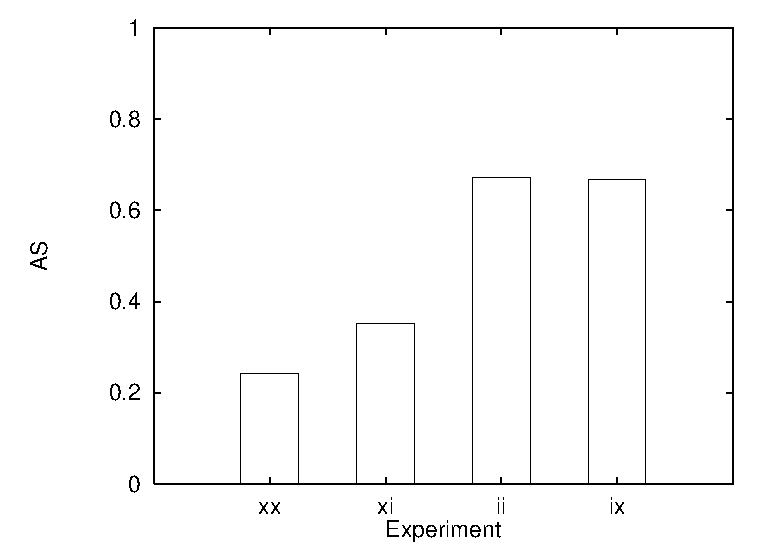
\includegraphics[width=5.5cm]{feedback/as.eps}}
\subfigure[DS]{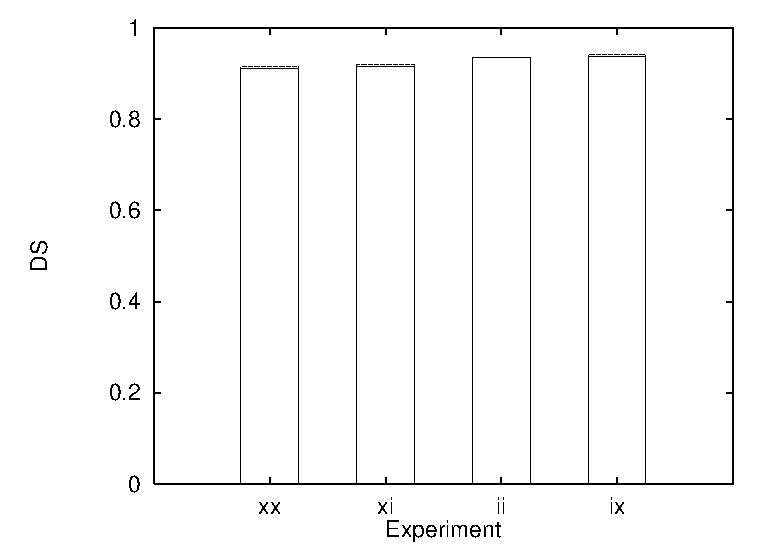
\includegraphics[width=5.5cm]{feedback/ds.eps}}\\
\subfigure[S]{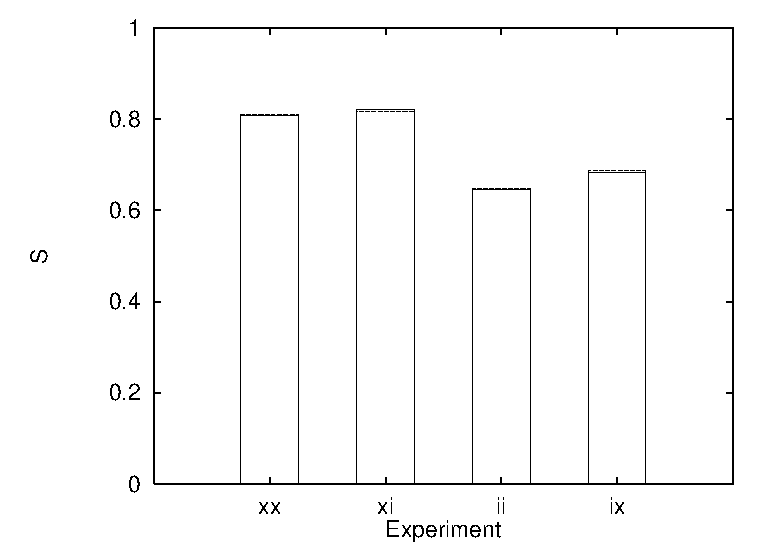
\includegraphics[width=5.5cm]{feedback/s.eps}}
\subfigure[D]{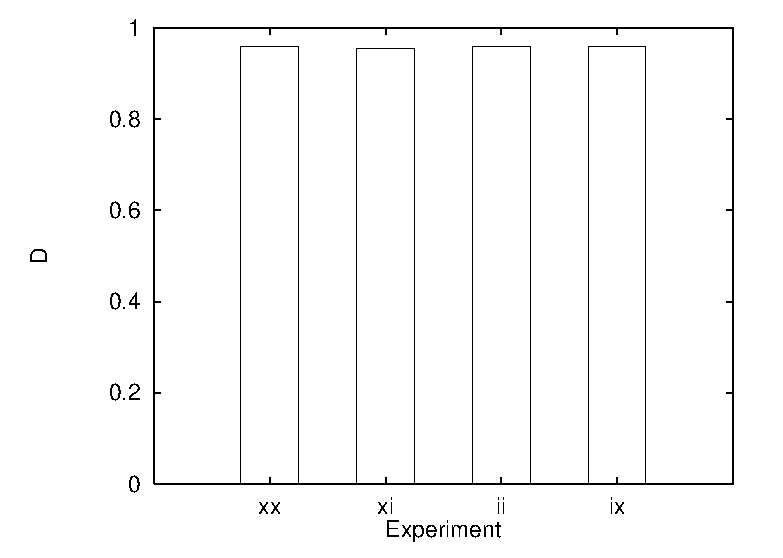
\includegraphics[width=5.5cm]{feedback/d.eps}}\\
\subfigure[C]{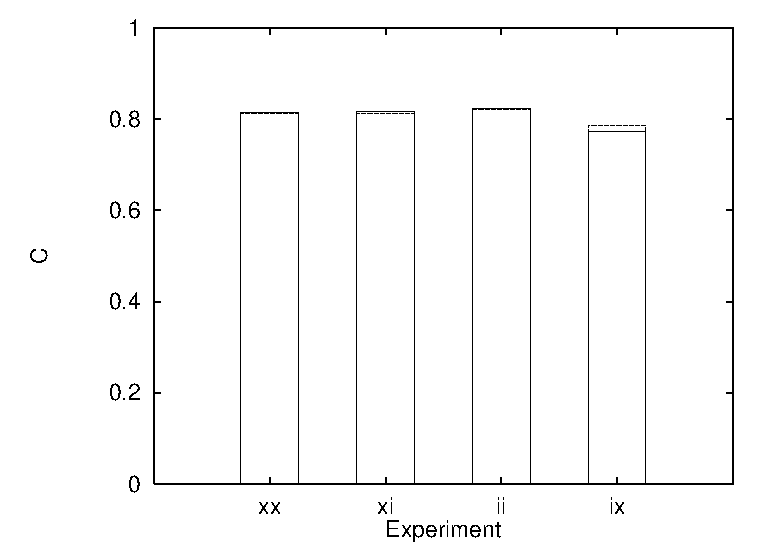
\includegraphics[width=5.5cm]{feedback/c.eps}}
\subfigure[P]{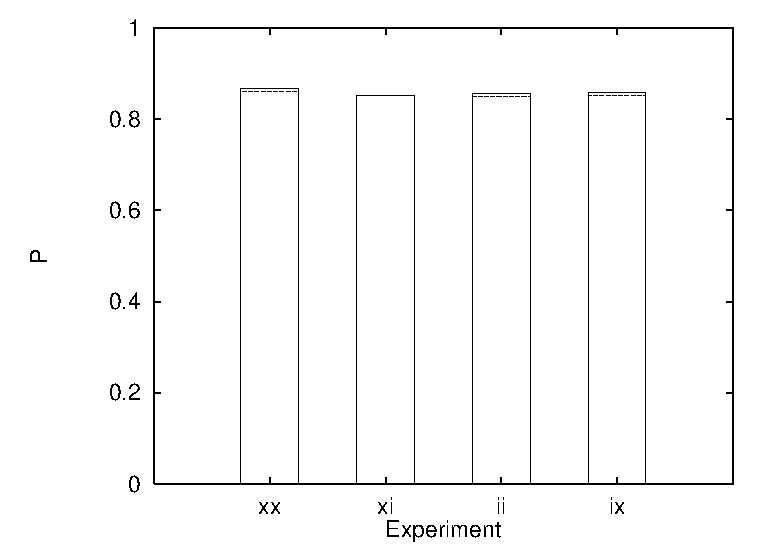
\includegraphics[width=5.5cm]{feedback/p.eps}}
\end{figure}
\begin{figure}[t]
\centering
\subfigure[CS]{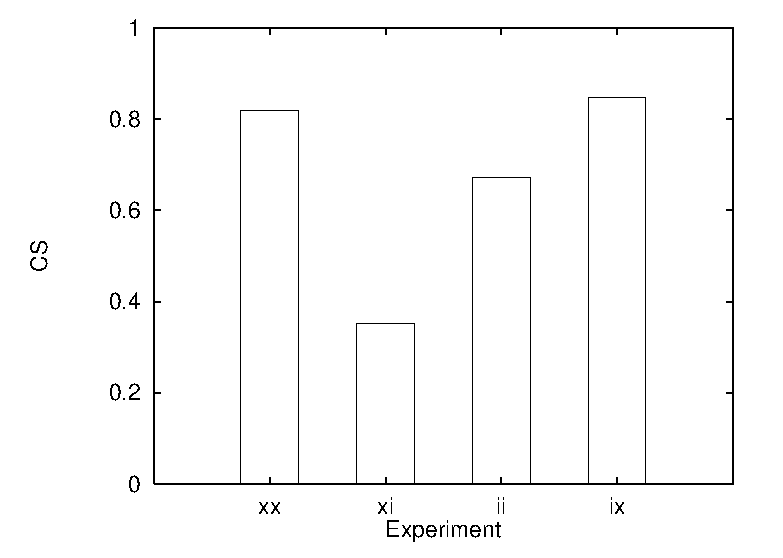
\includegraphics[width=5.5cm]{feedback/cs.eps}}
\caption{The results of experimenting with the different types of language games. Note that the first plot (a) shows the actual success, while the communicative success is plotted in the last Figure (f).}
\label{f:par:feedback}
\end{figure}


\begin{table}
\centering
\begin{tabular}{ld{3}@{~}c@{~}d{3}d{3}@{~}c@{~}d{3}d{3}@{~}c@{~}d{3}d{3}@{~}c@{~}d{3}} 
\lsptoprule
&     \multicolumn{3}{c}{{\bf xx}} & \multicolumn{3}{c}{{\bf xi}} & \multicolumn{3}{c}{{\bf ii}} & \multicolumn{3}{c}{{\bf ix}} \\\midrule
CS&   0.818 & $\pm$ & 0.006& 0.351 & $\pm$ & 0.010&        0.671 & $\pm$ & 0.004&  0.847 & $\pm$ & 0.003\\%\hline
AS&   0.241 & $\pm$ & 0.008& 0.351 & $\pm$ & 0.010&        0.671 & $\pm$ & 0.004&  0.667 & $\pm$ & 0.003\\%\hline
DS0&  0.912 & $\pm$ & 0.004& 0.916 & $\pm$ & 0.004&        0.935 & $\pm$ & 0.002&  0.937 & $\pm$ & 0.001\\%\hline
DS1&  0.915 & $\pm$ & 0.005& 0.920 & $\pm$ & 0.004&        0.936 & $\pm$ & 0.002&  0.941 & $\pm$ & 0.004\\%\hline
D0&   0.959 & $\pm$ & 0.000& 0.956 & $\pm$ & 0.002&        0.959 & $\pm$ & 0.000&  0.960 & $\pm$ & 0.000\\%\hline
D1&   0.958 & $\pm$ & 0.000& 0.955 & $\pm$ & 0.002&        0.960 & $\pm$ & 0.000&  0.960 & $\pm$ & 0.001\\%\hline
P0&   0.866 & $\pm$ & 0.002& 0.852 & $\pm$ & 0.004&        0.856 & $\pm$ & 0.001&  0.858 & $\pm$ & 0.002\\%\hline
P1&   0.860 & $\pm$ & 0.003& 0.851 & $\pm$ & 0.002&        0.851 & $\pm$ & 0.002&  0.851 & $\pm$ & 0.000\\%\hline
S0&   0.808 & $\pm$ & 0.031& 0.822 & $\pm$ & 0.017&        0.647 & $\pm$ & 0.046&  0.684 & $\pm$ & 0.144\\%\hline
S1&   0.810 & $\pm$ & 0.031& 0.817 & $\pm$ & 0.011&        0.647 & $\pm$ & 0.045&  0.688 & $\pm$ & 0.132\\%\hline
C0&   0.814 & $\pm$ & 0.005& 0.816 & $\pm$ & 0.008&        0.823 & $\pm$ & 0.037&  0.772 & $\pm$ & 0.117\\%\hline
C1&   0.812 & $\pm$ & 0.005& 0.811 & $\pm$ & 0.007&        0.821 & $\pm$ & 0.026&  0.787 & $\pm$ & 0.099\\%\hline
\lspbottomrule
\end{tabular}
\caption{The experimental results of the XSL game (xx), the guessing game (xi), the ostensive game (ii) and the observational game (ix).}
\label{t:par:feedback}
\end{table}

The ostensive game and the observational game appear to be much better than the guessing game. This increase in the performance is measured by the actual success,\footnote{The communicative success of the observational game is much higher because this is measured when both robots `think' they are successful. This happens when both robots identified a form-meaning association consistent with their categorisation. It is independent of whether both robots referred to the same referent.} which is almost 30 \% (!) better ($p=0.0000$). However, the specificity is much lower: 0.18 for experiment {\bf ii} and 0.14 in {\bf ix} ($p=0.0000$). This low specificity indicates that the lexicon is not stable and it must bear much polysemy.

The difference in consistency of the observational game is insignificant ($p>1$). The consistency of {\bf ii} is hardly different than the basic experiment. Note that the standard deviations of experiment {\bf ix} is about 0.1 for both the specificity as the consistency. The results of the experiments vary a lot from run to run. The worst run has a consistency of 0.401, whereas the best one has 0.856. The basic experiment had all its values in between and a standard deviation of 0.007. Similar findings are also valid for {\bf ii} that has standard deviation of about 0.05 for the specificity and 0.03 for consistency.

The discriminative success of {\bf ix} and {\bf ii} is slightly higher than the basic experiment ($p=0.0000$), but this has to do with the higher communicative success, which influence the discriminative success. The differences of D and P are both small and insignificant.

\subsection{Discussion}

When looking at the results, some important observations can be made. A language game needs some extra-linguistic information. As expected, no effective lexicon gets off the ground in the XSL game. 

It seems that in the guessing game, a more informative lexicon emerges. It is more informative because the specificity and consistency are higher than in the ostensive- and observational games. More information seems to have a cost in these experiments, namely a lower actual success. The actual success of the games that incorporate joint attention, on the other hand, is high. This also has a cost, namely a lower specificity.

\begin{figure}[t]
\centerline{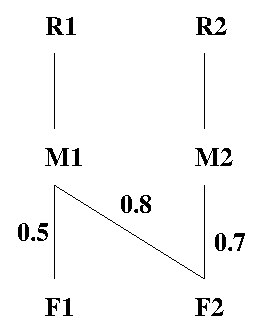
\includegraphics[width=3cm]{feedback/example.eps}}
\caption{The semiotic landscape of one agent in the example that is described in the text.}
\label{f:par:example}
\end{figure}


To understand why the experiments that use joint attention have higher actual success and lower specificity (and to some extend consistency), it is instructive to look at an example: Suppose a robot has a (part of a) lexicon as in \figref{f:par:example}. If the robot is a speaker and R1 is the topic, it would select F2 as the utterance independent of the type of game.\footnote{Remember that the guessing game is compared with both the ostensive and observational game, since what is important is the joint attention.} If R2 is the topic, it would also select F2. Remember that the robots select the associations that have highest scores.

Suppose that this robot is a hearer, and it hears F2. If the robot plays a guessing game, it would select M1 and consequently R1 will be its topic. If however, the speaker intended to name R2, the game is a failure; there is a mismatch in referent. The score $\sigma_{M1F2}$ between M1 and F2 is decreased.

But now suppose that the robot plays observational- or ostensive games. If the speaker's topic is R2, the hearer will also have R2 as its topic, conform the joint attention principle. If the hearer now hears F2, it will select M2 as its meaning (since this categorises the only potential topic) and the language game is a success. Not only communicative, but also actual. Now the scores are adapted as follows: $\sigma_{M2F2}$ is increased and $\sigma_{M1F2}$ is decreased.

If such games will continue for a while, there will ideally emerge a preference where R2 is named with F2 and R1 with F1. But if, at some point before this happens, the robot is again the speaker and it chooses to name R1. It will still choose F2 to name M1.  If a guessing game is played, there is a reasonable chance that the game ends in failure. The hearer (i.e. the other robot not shown in the figure) will have a similar but not equal competition of association scores and it might already be at the point where F2 will preferably be interpreted with meanings categorising R2. So, the speaker will decrease $\sigma_{M1F2}$. When, on the other hand, an observational game is played, and the robot names R1 with F2, it is very likely that the game will end in success. This is because the hearer knows what the topic is. So, if it as an association where F2 relates to some meaning M which categorises R1, the game is a success. As a consequence the association score $\sigma_{M2F2}$ of the speaker increases again, whereas competing association scores decrease. The attempt to disambiguate F2 in favour of R2 has to start again.

This way the observational game allows more polysemy, yielding lower specificity. The same argument holds for the ostensive game. Since the robots easily establish actual success this way, the actual success is relatively high. So, it seems that establishing joint attention decreases the pressure to exploit the complete space of possibilities during selection. This is not surprising since joint attention makes linguistic communication redundant.

\index{guessing game|)}
\index{ostensive game|)}
\index{XSL game|)}
\index{feedback|)}
\index{joint attention|)}

\section{The Observational Game}\label{s:par:observ}\label{s:feed:oli}

In the previous section, an experiment with the observational game has been presented. It has been observed and explained that the specificity is low. So, the lexicon is unstable and allows much referential polysemy and some synonymy. But since the actual success is high, it is interesting to see whether it is possible to achieve good results for specificity and consistency as well. 

While looking for working implementations it also has been found that lateral inhibition is a crucial source of lexicon development. This is conform witht the findings of \citet{oliphant:1997}, \citet{steels:2000}, \citet{dejong:2000} and \citet{kaplan:2000}. To investigate this a variant of the observational game of the previous section is presented in which lateral inhibition is absent.

\subsection{The Experiments}

The experiments are compared with the observational game.

\begin{description}
\item[ix$_p$] Creation probability. In all experiments up to now, the word-form creation probability has been $P_s=0.02$. In this experiment $P_s=0.4$. This way the speaker is less modest in inventing new word-forms when it cannot produce an utterance. \index{form!creation probability}
\item[ix$_{li}$] Lateral inhibition. In this experiment lateral inhibition of the association scores is not used. So, when an observational game is considered successful by the robots. This happens when either robot performed a communication act, and hence it need not be actually successful. In that case, only the ``winning'' association score is increased. All other scores are unaltered. For the rest this experiment is equal to experiment {\bf ix}. \index{lateral inhibition}
\end{description}

\subsection{The Results}

The results are presented in \tabref{t:par:observ} and \figref{f:par:observ}, where experiments {\bf ix$_p$} and {\bf ix$_{li}$} are compared with the observational game ({\bf ix}) presented in the previous section.

\begin{figure}
\centering
\subfigure[AS]{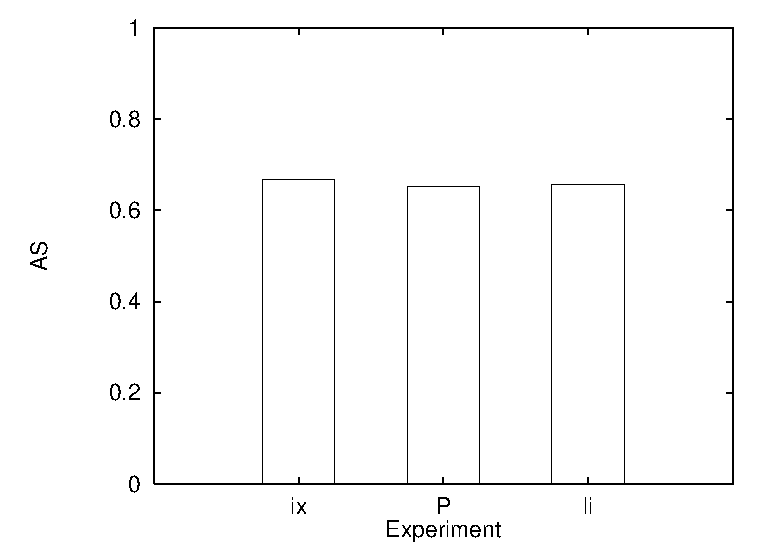
\includegraphics[width=5.5cm]{feedback/as0.eps}}
\subfigure[DS]{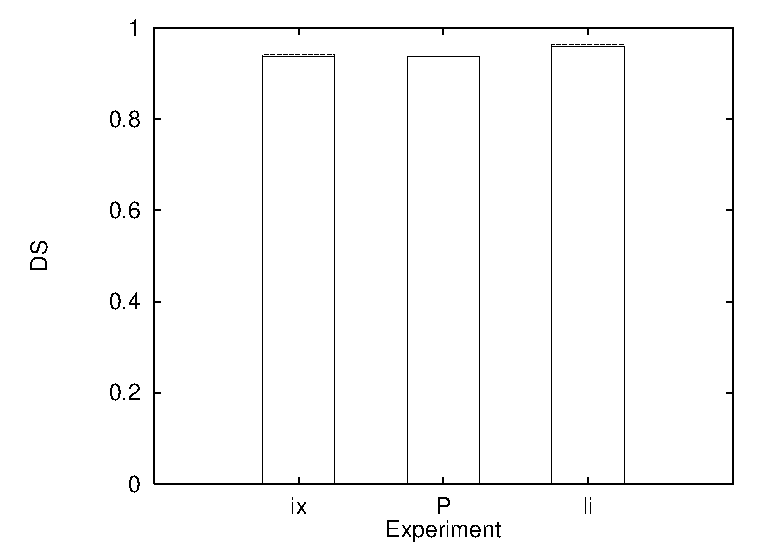
\includegraphics[width=5.5cm]{feedback/ds0.eps}}\\
\subfigure[S]{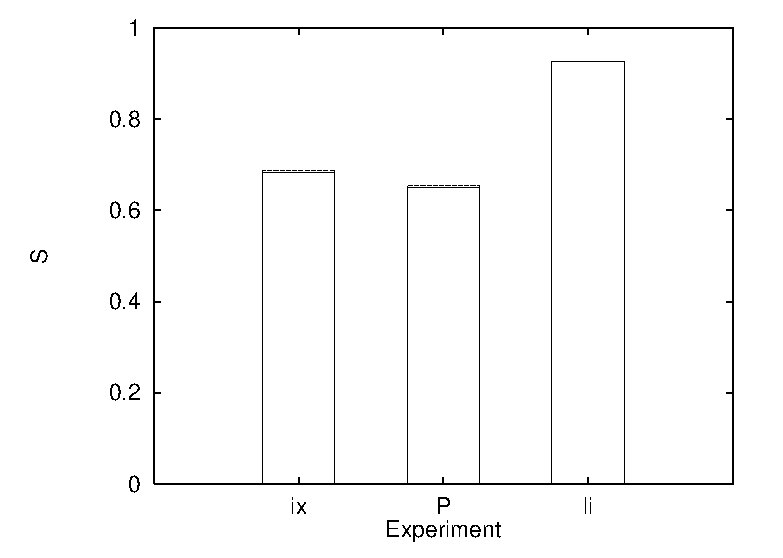
\includegraphics[width=5.5cm]{feedback/s0.eps}}
\subfigure[D]{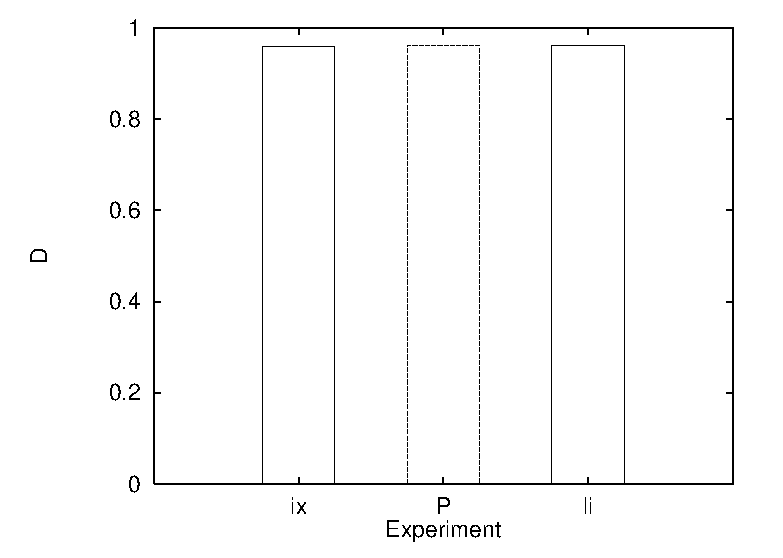
\includegraphics[width=5.5cm]{feedback/d0.eps}}\\
\subfigure[C]{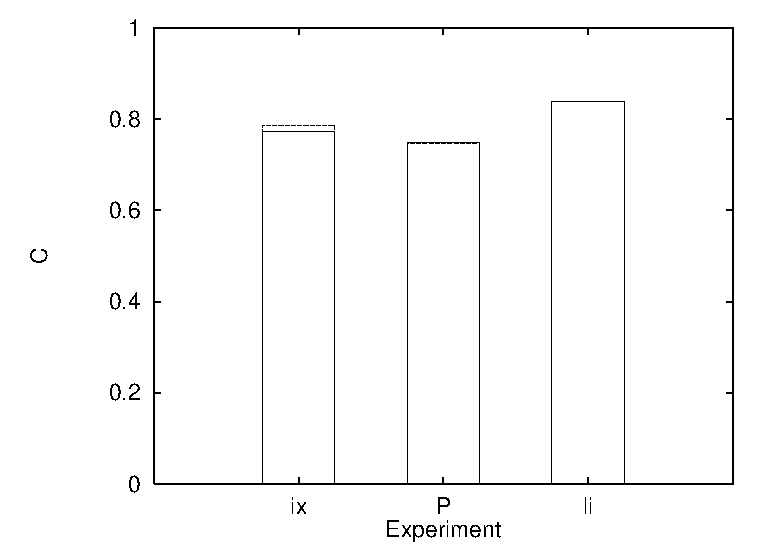
\includegraphics[width=5.5cm]{feedback/c0.eps}}
\subfigure[P]{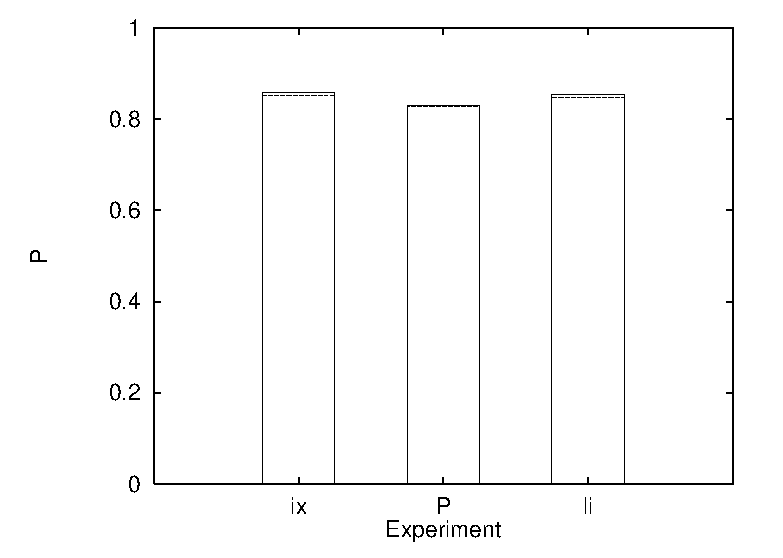
\includegraphics[width=5.5cm]{feedback/p0.eps}}
\end{figure}
\begin{figure}[t]
\centering
\subfigure[CS]{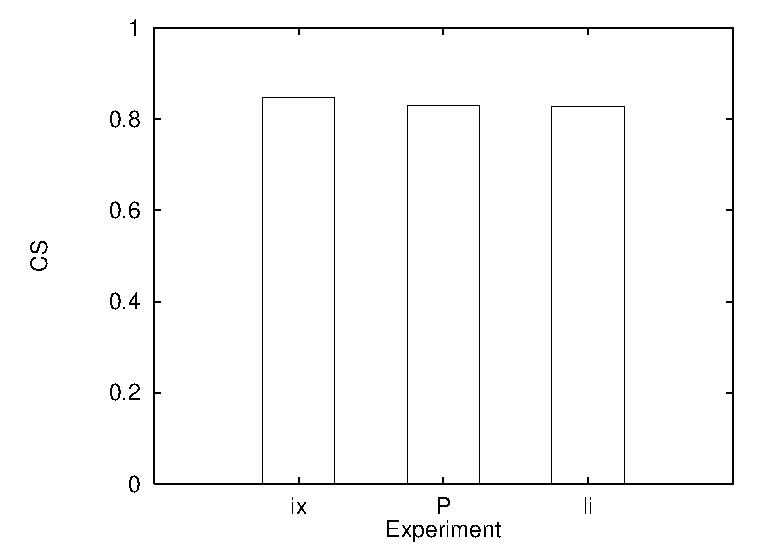
\includegraphics[width=5.5cm]{feedback/cs0.eps}}
\caption{The results of experimenting with different observational games.}
\label{f:par:observ}
\end{figure}


\begin{table}
\centering
\begin{tabular}{ld{3}@{~}c@{~}d{3}d{3}@{~}c@{~}d{3}d{3}@{~}c@{~}d{3}}
\lsptoprule
& \multicolumn{3}{c}{{\bf ix}}& \multicolumn{3}{c}{{\bf ix$_p$}} & \multicolumn{3}{c}{{\bf ix$_{li}$}} \\\midrule
CS&  0.847 & $\pm$ & 0.003& 0.827 & $\pm$ & 0.005& 0.830 & $\pm$ & 0.001\\%\hline 
AS&  0.667 & $\pm$ & 0.003& 0.657 & $\pm$ & 0.005&0.651 & $\pm$ & 0.002\\%\hline 
DS0& 0.937 & $\pm$ & 0.001& 0.960 & $\pm$ & 0.001&0.937 & $\pm$ & 0.003\\%\hline 
DS1& 0.941 & $\pm$ & 0.004& 0.963 & $\pm$ & 0.001&0.936 & $\pm$ & 0.003\\%\hline 
D0&  0.960 & $\pm$ & 0.000& 0.960 & $\pm$ & 0.000&0.960 & $\pm$ & 0.001\\%\hline
D1&  0.960 & $\pm$ & 0.001& 0.961 & $\pm$ & 0.001&0.961 & $\pm$ & 0.000\\%\hline 
P0&  0.858 & $\pm$ & 0.002& 0.853 & $\pm$ & 0.001&0.830 & $\pm$ & 0.001\\%\hline 
P1&  0.851 & $\pm$ & 0.000& 0.848 & $\pm$ & 0.001&0.827 & $\pm$ & 0.000\\%\hline 
S0&  0.684 & $\pm$ & 0.144& 0.927 & $\pm$ & 0.002&0.617 & $\pm$ & 0.094\\%\hline 
S1&  0.688 & $\pm$ & 0.132& 0.927 & $\pm$ & 0.002&0.622 & $\pm$ & 0.095\\%\hline 
C0&  0.772 & $\pm$ & 0.117& 0.838 & $\pm$ & 0.003&0.709 & $\pm$ & 0.114\\%\hline 
C1&  0.787 & $\pm$ & 0.099& 0.839 & $\pm$ & 0.003&0.707 & $\pm$ & 0.112\\%\hline 
\lspbottomrule
\end{tabular}
\caption{The results of the variants of the observational game.}
\label{t:par:observ}
\end{table}

For experiment {\bf ix$_p$} the communicative success and actual success are more or less similar as in the experiment of the previous section, and so are the distinctiveness and parsimony. The difference in consistency is not very significant ($p=0.1432$). The discriminative success is about 2.5 \% higher when $P_s=0.4$ ($p=0.0000$). This however, is an artefact of the method for calculating the discriminative success. Because the speaker invents forms more often, the hearer plays discrimination games more often. Recall that the hearer only categorises when it receives an utterance. Since the discriminative success is a function of language games rather than of the discrimination games, the discriminative success is higher.

\begin{figure}[t]
\centering
\subfigure[{\bf ix}]{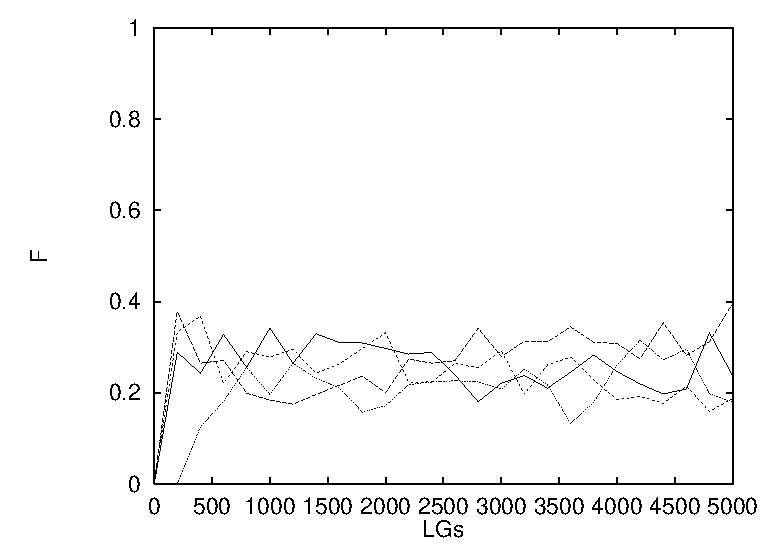
\includegraphics[width=5.5cm]{feedback/fr0-0.eps}}
\subfigure[{\bf ix$_p$}]{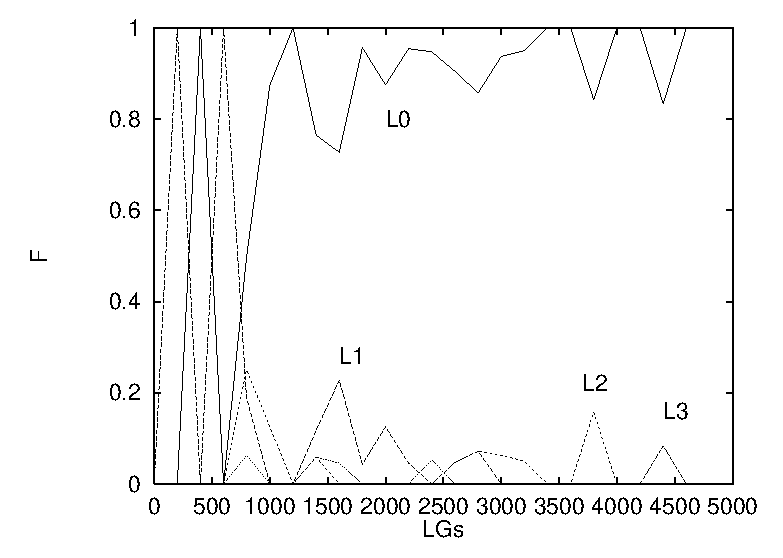
\includegraphics[width=5.5cm]{feedback/fr0-4olib.eps}}
\caption{The form-referent competitions of experiments {\bf ix} (preceding section) and {\bf ix$_p$} for some form.}
\label{f:par:FR-comp}
\end{figure}

More important for experiment {\bf ix$_p$} is the increase of specificity by 0.24 ($p=0.0000$). Apparently the system reduces polysemy when $P_s$ is higher. This is nicely shown by the form-referent competition diagrams of the two experiments (\figref{f:par:FR-comp}). These diagrams show the competition for a word-form that is used very frequently in both experiments. The two diagrams clearly show the difference between experiment {\bf ix} and {\bf ix$_p$}. The word-form of experiment {\bf ix} is used for all four referents almost equally often. The word-form displayed for {\bf ix$_p$} clearly evolves to name L0 pretty stable and specific.


The experiment where lateral inhibition is absent, also most measures are similar to {\bf ix} from the previous section. However, both specificity and coherence is lower than in experiment {\bf ix}. Hence when there is no lateral inhibition, more polysemy and synonymy emerges in the system.

\subsection{Discussion}

When the creation probability is higher, specificity is also higher. This can be explained as follows: When $P_s$ is low, and the speaker cannot name some meaning, the probability is high that it will not invent a new word-form. This leaves the meaning unassociated, which increases the likelihood that the meaning will be associated with an already existing word-form. This may happen in a later game by means of word-form adoption when the robot is hearer. This way the word-form increases its amount of one-to-many mappings and apparently its polysemy as well. When the $P_s$ is higher, this effect is less. Thus increasing the specificity.


It is interesting to note that the high average actual success is likely to be mainly caused by the joint attention mechanism and the easiness of establishing communicative success when joint attention is used. Note that, like in the ostensive game, joint attention makes the linguistic communication redundant. The ostensive game does not differ very much from the observational game. The feedback that it provides is more or less the same information that is provided by the joint attention mechanism.

Recall that the potential understandability is approximately 79 \%. When multiplying this value with the average communicative success of approximately 83~\%, this yields 66 \% which corresponds nicely to the average actual success. So, it appears that the difference between communicative success and actual success is caused by the inability of the robots to construct a coherent context as explained in \chapref{ch:lg}. This indicates that there are still other mechanisms that are responsible for the imperfect communication.


The observational game is inspired by the experiments done by Mike \citet{oliphant:1997,oliphant:1998,oliphant:2000}, although they are not exactly the same. A big first difference is inherent on the use of robots. \index{Oliphant, Mike}

Oliphant's agents have access to both the signal and the meaning of it during a language game, which he calls observation. The learning mechanism tries to converge an ideal communication system based on the word-meaning associations. This is also done in our experiments. However, the robots have, in principle, no access to the meaning of a signal other than to its referent. Another difference is in the learning algorithm (or the update of the scores). Where Oliphant uses a.o. Hebbian- and Bayesian learning, a different update rule is used here.

It is clear that the robots can ground a reasonable communication system with a reasonable success without the availability of feedback. This, however only works when joint attention is established and the word-form creation rate is sufficiently high. This confirms the work of Mike \citet{oliphant:1997} and Edwin \citet{dejong:2000}. De Jong also showed in simulations that the naming game needs no feedback on the effect of a game. Like \citet{oliphant:1997}, Luc \citet{steels:2000} and Fr\'ed\'eric \citet{kaplan:2000}, De Jong argues that lateral inhibition is an essential ingredient for the success. The experiment without lateral inhibition again confirmed this finding. Without lateral inhibition all competing associations can be strengthened in successful games. So, the competition between form-meaning associations is less effective. It is left as an exercise for the reader to invent an example.

\index{observational game|)}

\section{Word-form Creation}\label{s:par:ps}
\index{form!creation probability|(}

As has been observed in the previous section, the word-form creation probability $P_s$ may have an enormous impact on the lexicon formation. In the basic experiment $P_s=0.02$, which is a setting based upon earlier experiments \citep{vogt:1998b}. In this section, the influence if the word-form creation probability is investigated more structurally.

\subsection{The Experiments}

The creation probability is varied over 11 experiments.

\begin{description}
\item[$P_s$] $P_s$ is varied from 0.0 to 1.0 with intermediate steps of 0.1. The experiments further implement the guessing game and is therefore a variant of the basic experiment.
\end{description}

\subsection{The Results}

\begin{figure}
\centering
\subfigure[CS]{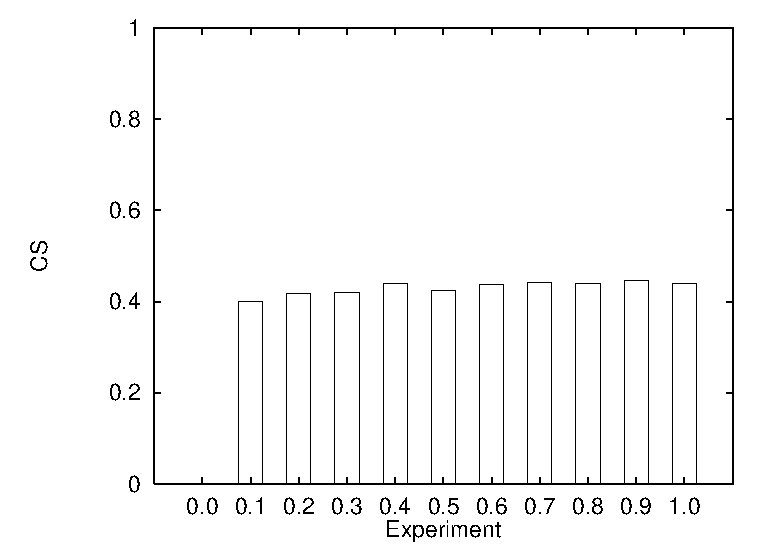
\includegraphics[width=5.5cm]{lexicon/cs_p.eps}}
\subfigure[DS]{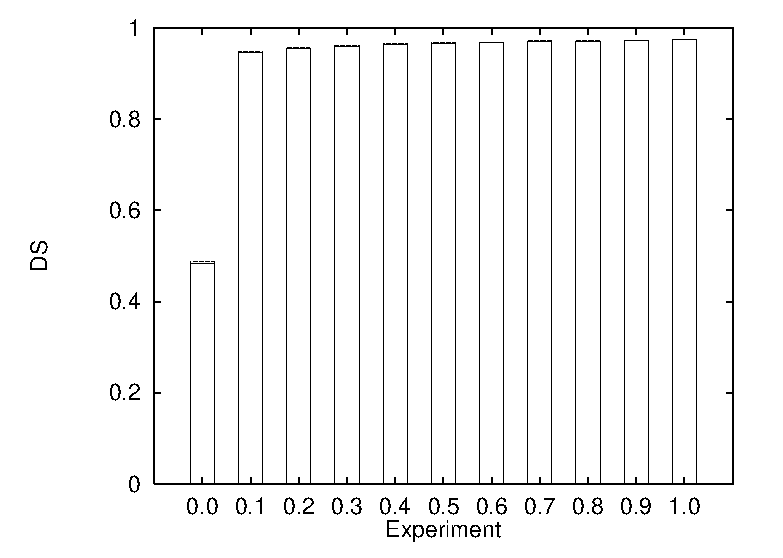
\includegraphics[width=5.5cm]{lexicon/ds_p.eps}}\\
\subfigure[S]{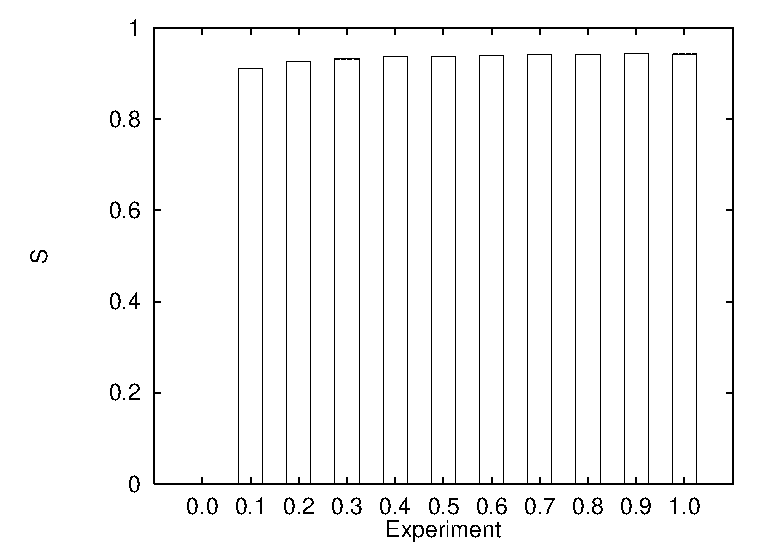
\includegraphics[width=5.5cm]{lexicon/spec_p.eps}}
\subfigure[D]{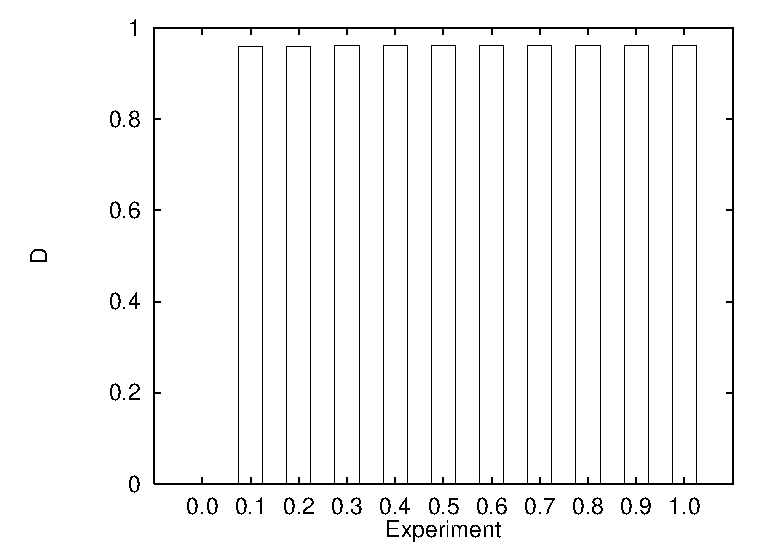
\includegraphics[width=5.5cm]{lexicon/dist_p.eps}}\\
\subfigure[C]{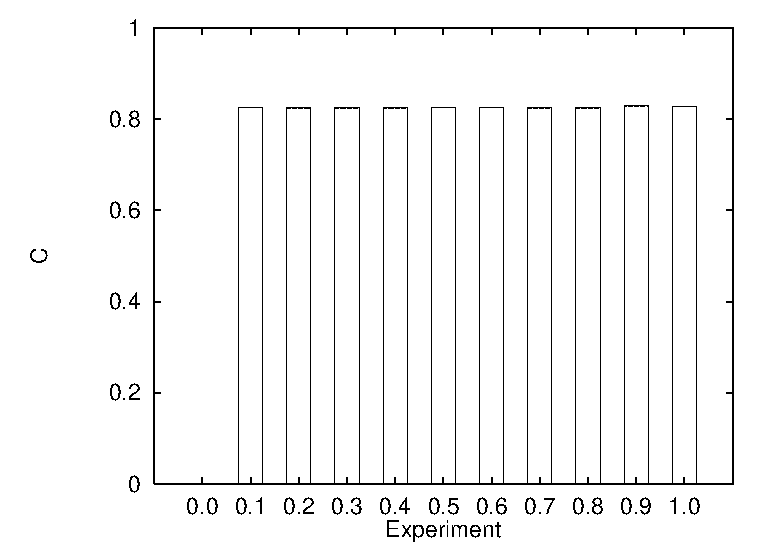
\includegraphics[width=5.5cm]{lexicon/cons_p.eps}}
\subfigure[P]{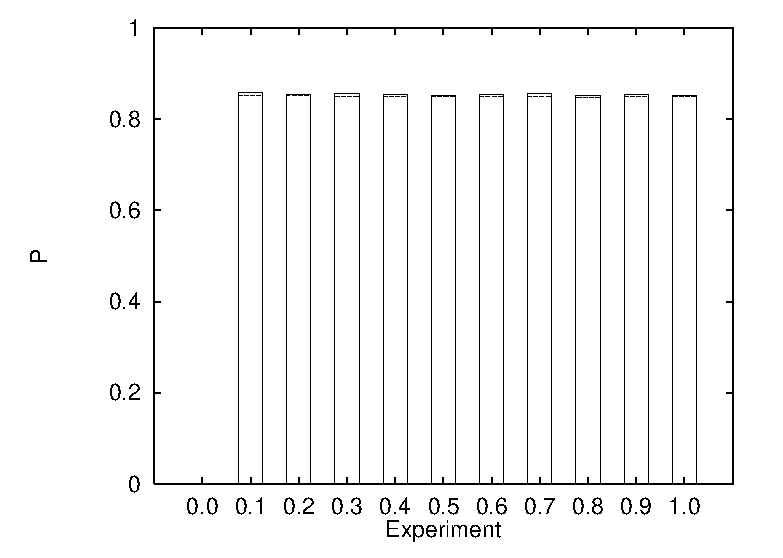
\includegraphics[width=5.5cm]{lexicon/pars_p.eps}}
\caption{The results of a series experiments where creation probability $P_s$ is varied from 0 to 1 with steps of 0.1.}
\label{f:lex:p}
\end{figure}

The results are shown in \figref{f:lex:p}. It is trivial that the communicative success, specificity, distinctiveness, consistency and parsimony are 0 when $P_s=0$. When no word-forms are created no communication can take place. All mentioned measures are only calculated when linguistic communication took place. The discriminative success is approximately 50 \% because only the speaker now performs a discrimination game and the discriminative success is calculated as an average discriminative success per {\em language game}. Since the robots can in principle discriminate almost perfectly (see \figref{f:st:ds}, page \pageref{f:st:ds}), the discriminative success is almost 50 \%. 

Figure \ref{f:lex:p} shows that there is hardly any difference in the experiments when $P_s$ is varied between 0.1 and 1. The discriminative success and specificity are slightly increasing, as it appears monotonically. The communicative success also seems to be increasing, but it also shows some local minima and maxima. It seems that when $P_s=0.9$, the communicative success is highest, but when $P_s=0.4$, the communicative success is second best. There does not seem to be a relation. distinctiveness, consistency and parsimony seem to be indifferent for the variation of $P_s$.

When $0.1 \leq P_s \leq 1.0$, then the system outperforms the basic experiment. Although distinctiveness, parsimony and consistency are more or less the same as in the basic experiment; the communicative success is about 5 -- 9 \% higher, discriminative success is 4 \% higher and specificity is approximately 0.09 higher. All these differences are significant ($p=0.0000$).

\begin{figure}[t]
\centerline{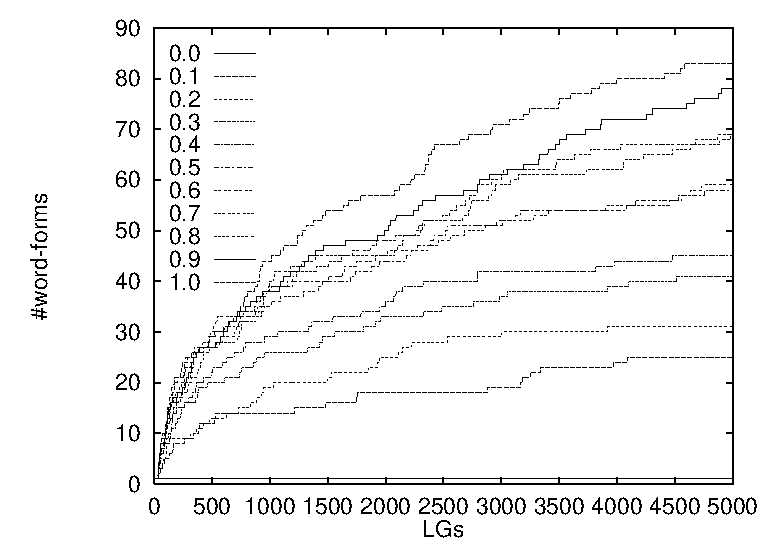
\includegraphics[width=12cm]{lexicon/words.eps}}
\caption{The lexicon growth for different values of the creation probability $P_s$, which is varied from 0 to 1 with steps of 0.1.}
\label{f:lex:words}
\end{figure}

It is interesting now to see how the number of words grow in the communication system. Figure \ref{f:lex:words} shows the growth of the number of word-forms that are used successfully in the experiments. It is clear that the number of word-forms grows faster when the creation probability increases. Recall that the number of word-forms in the basic experiment grew to only 8 word-forms. When $P_s=0.1$ this already increases to 25 word-forms, and when $P_s=1.0$ there emerge more than 80 word-forms. As a comparison, the basic experiment finished with 12 word-forms. Remember that there are only 4 referents in the robots' environment!

\subsection{Discussion}

The small differences between the results when $P_s=00.1$ and $P_s=1.0$ has also been observed in simulations on the naming game \citep{kaplan:2000}.

\index{synonymy}From \figref{f:lex:words} it can be inferred that the rate of synonymy thus increases very much, although this is not obvious from the consistency.\footnote{Recall that consistency is weighted over the frequency of occurrences of referent-word-form pairs.} However, the robots do significantly better in learning to commentate than when $P_s=0.02$ as in the basic experiment. This may be a side effect of the fact the agents optimise their lexicons for word-meaning associations rather than word-referent associations. When there are more word-forms, there is less need for many-to-many relations at the form-meaning level. But due to the fact that there is a high level of one-to-many relations between referent and meaning, synonymy is also relatively high.

As also observed in the previous section, the specificity is higher when $P_s$ is higher. This is not surprising, since there are more word-forms to name the different meanings, thus decreasing the level of one-to-many relations between form and meaning. And since the different meanings are distinctive to a high degree, these word-forms refer to a unique referent more and more. A higher creation probability also yields a higher communicative success. The cost however of a higher creation probability is that there are more word-forms to name the same number of referents.
\index{form!creation probability|)}

\section{Varying the learning rate}\label{s:par:lr}
\index{learning rate|(}

The adaptation scores are adapted using a walking average. These scores are adapted for the category scores $\nu$, the effectiveness scores $\rho$ and the association scores $\sigma$ (\chapref{ch:lg}). The formula by which the scores $s$ are adapted is repeated here for clarity:
\begin{eqnarray}
s = \eta \cdot s' + (1-\eta)\cdot X
\end{eqnarray}


where $\eta$ is the learning rate and $X$ is the success factor. The type of score is dependent on the game being played and so is $X$. This equation is used to update category-, effectiveness- and association scores.

In the basic experiment, the learning rate has been set to $\eta=0.99$. This score has been chosen to be this value based upon early experiments, which was before the current implementation has been finished. What would happen if $\eta$ is varied.

\subsection{The Experiments}

The experiments implement the guessing game.

\begin{description}
\item[$\eta$] Learning rate. The learning rate is varied from 0.0 to 1.0 with steps of 0.1.
\end{description}

\subsection{The Results}

\begin{figure}
\centering
\subfigure[CS]{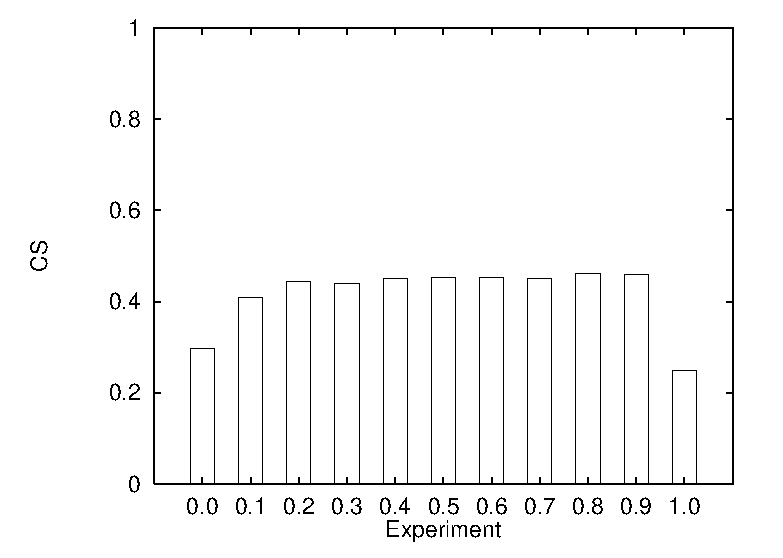
\includegraphics[width=5.5cm]{lexicon/cs_A.eps}}
\subfigure[DS]{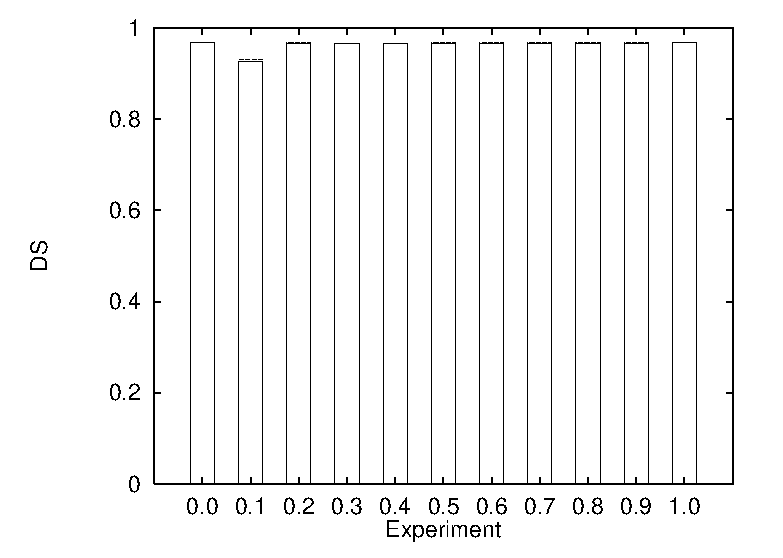
\includegraphics[width=5.5cm]{lexicon/ds_A.eps}}\\
\subfigure[S]{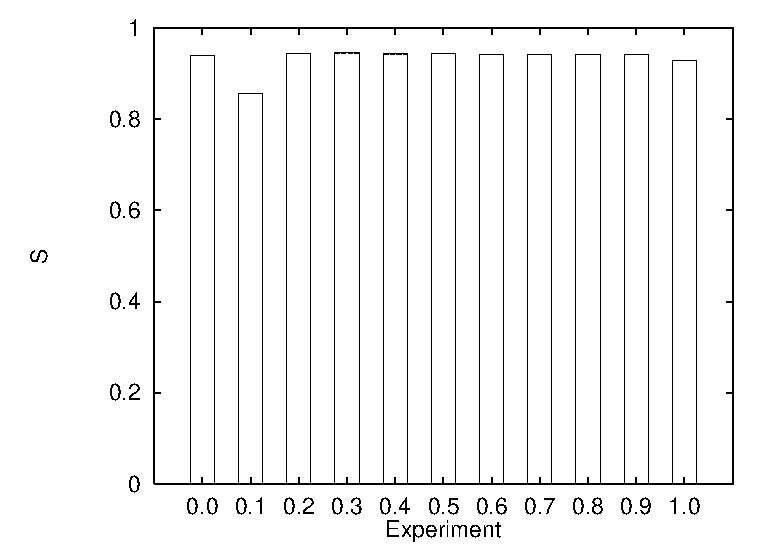
\includegraphics[width=5.5cm]{lexicon/spec_A.eps}}
\subfigure[D]{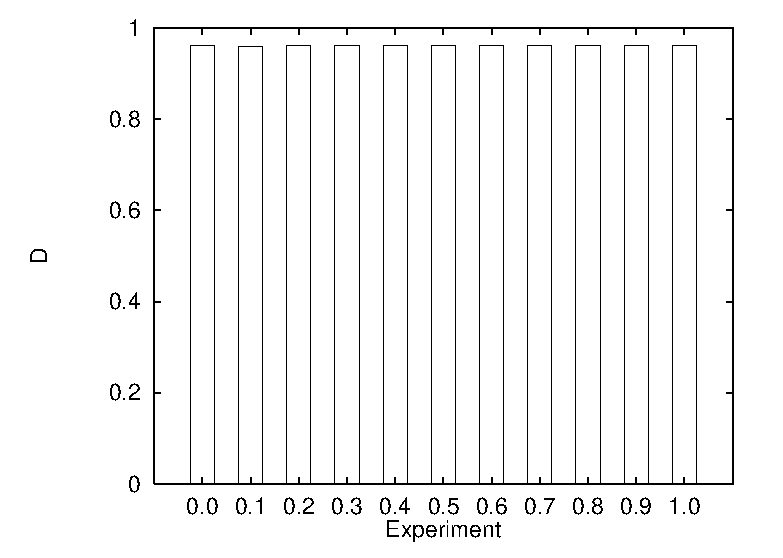
\includegraphics[width=5.5cm]{lexicon/dist_A.eps}}\\
\subfigure[C]{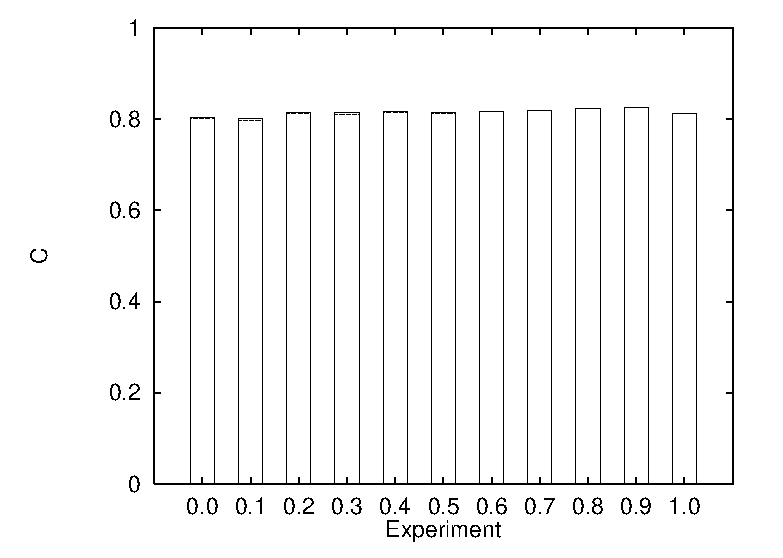
\includegraphics[width=5.5cm]{lexicon/cons_A.eps}}
\subfigure[P]{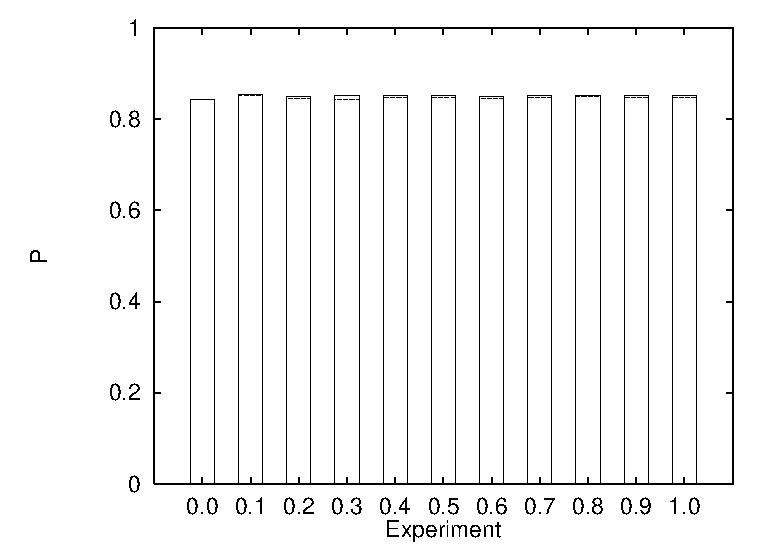
\includegraphics[width=5.5cm]{lexicon/pars_A.eps}}
\caption{The results of a series of experiments where the learning rate $\eta$ has been varied from 0 to 1 with intervals of 0.1.}
\label{f:lex:A}
\end{figure}

Figure \ref{f:lex:A} shows the results of these experiments. The experiments where $\eta=0$ and $\eta=1$ perform very poor, poorer than in the basic experiment ($p=0.0000$ in both cases). If $\eta=0$, the scores are completely dependent from the previous language game where the element is used. When $\eta=1$ the scores are not updated at all. Obviously, taking only the last game into account, the robots cannot learn the communication system properly. Neither can it be learned when the scores are not updated. The communicative success when $\eta=1$ is about 5 \% lower than when $\eta=0$ ($p=0.0000$). So, taking only the last game into account is better than doing nothing. Figure \ref{f:lex:csA0} shows that these communication systems no longer learn after game 500. That some games are successful is caused by the fact that form-meaning associations do get formed as normal and the rest is more or less coincidence.

\begin{figure}[t]
\centering
\subfigure[$\eta=0$]{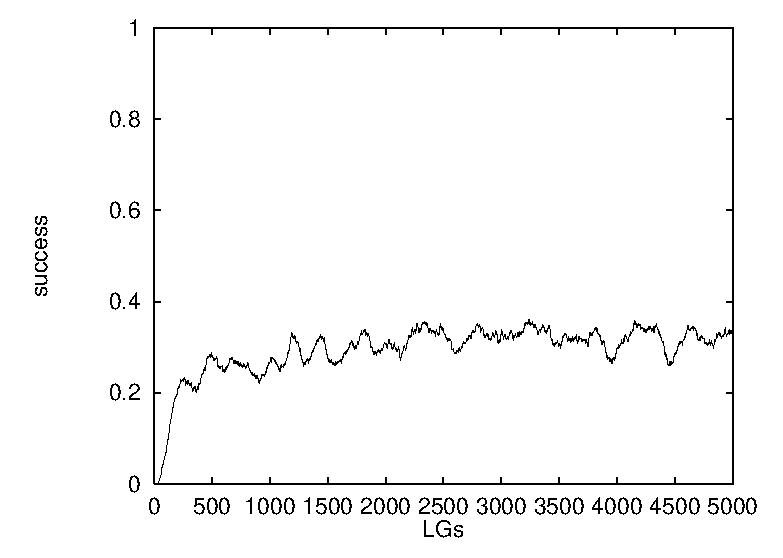
\includegraphics[width=5.5cm]{lexicon/csA0.eps}}
\subfigure[$\eta=1$]{\includegraphics[width=5.5cm]{lexicon/csA1.eps}}
\caption{The evolution of the communicative success when (a) $\eta=0$ and (b) $\eta=1$. It is clear that the communication system is not learned.}
\label{f:lex:csA0}
\end{figure}

When $\eta=0.1$, the communicative success is higher than in the basic experiment ($p=0.0000$), but it is lower than when $0.2\leq\eta\leq0.9$ ($p=0.0000$ when compared to $\eta=0.2$). Furthermore, in this experiment the discriminative success and specificity are lower than when $0.2\leq\eta\leq0.9$ (again $p=0.0000$ when compared to $\eta=0.2$). Figure \ref{f:lex:csA01} shows however, that the communication is learned when $\eta=0.1$ as well as when $\eta=0.2$. It only takes longer, so the global averages are lower. Strangely enough the discriminative success and specificity are also lower when $\eta=0.1$ than when $\eta=0.0$.It is not understood why this is the case.

\begin{figure}
\centering
\subfigure[CS ($\eta=0.1$)]{\includegraphics[width=5.5cm]{lexicon/csA01.eps}}
\subfigure[CS ($\eta=0.2$)]{\includegraphics[width=5.5cm]{lexicon/csA02.eps}}\\
\subfigure[S ($\eta=0.1$)]{\includegraphics[width=5.5cm]{lexicon/specA01.eps}}
\subfigure[S ($\eta=0.2$)]{\includegraphics[width=5.5cm]{lexicon/specA02.eps}}\\
\subfigure[DS ($\eta=0.1$)]{\includegraphics[width=5.5cm]{lexicon/dsA01.eps}}
\subfigure[DS ($\eta=0.2$)]{\includegraphics[width=5.5cm]{lexicon/dsA02.eps}}
\caption{Comparing the communicative success, specificity and discriminative success in the cases where $\eta=0.1$ and $\eta=0.2$.}
\label{f:lex:csA01}
\end{figure}

 Figure \ref{f:lex:A} (a) shows that  when $0.2 \leq \eta \leq 0.9$ the communicative success seems to be increasing slightly. Differences, however are hardly significant. When comparing the case where $\eta=0.2$ with $\eta=0.9$, the difference has a significance of $p=0.0892$. Nevertheless, the increase really appears to be there. 

\subsection{Discussion}

The results showed that a successful lexicon cannot be learned when the scores are not adapted. Neither can it be learned when the memory of a past interaction lasts only one re-occurrence of the association.

It is surprising that the system develops more or less equally well when $\eta=0.2$ than when $\eta=0.9$. In the first case the last few interactions have much more influence on the selection than the complete history of interactions. When $\eta=0.9$ the vice versa is true. It is not clear why this is the case.


The results of this section show that the difference between the weight with which past success influences the experiment is high. When the learning rate $\eta$ varies between 0.1 and 0.9 the success of the language games is higher than when $\eta=0.99$. In that case the system is too much based on the past and as a result the system learns too slow.
\index{learning rate|)}


\section{Word-form Adoption}\label{s:par:adopt}
\index{form!adoption}

In the basic experiment the hearer only has to adopt a new word-form when it cannot find a matching form-meaning association. This happens when either the form is unknown to the hearer or when its meaning(s) do not match a distinctive category of a possible topic. In the Talking Heads, a word-form may also be adopted when there is a mismatch in referent \citep{steels:2000}. I.e. when the hearer did find a matching form-meaning, but the thus identified topic does not cohere with the speaker's topic. Intuitively, this strategy seems to be beneficial. If the hearer misinterprets the speaker, it should learn what the speaker meant.

\subsection{The Experiments}

Three experiments are done that investigate the impact from the extra word-form adoption. All experiments implement the guessing game. It differs from the basic experiment in that the uttered word-form is adopted by the hearer when the language game ends in a mismatch in referent. In that case the hearer identifies a topic. How this topic is selected is subject to variation. If this topic is not the same as the hearer identified before, the word-form is adopted according to the rules explained in \sectref{s:cm:ng}.

The three experiments vary in the way the topic is selected:

\begin{description}
\item[R] Random. The topic is selected at random, like is the case when the hearer adopts a word-form in the basic experiment.

\item[T] Correspondence. The topic is identified via the correspondence criterion, like is done when joint attention is established. This is only done when there is a mismatch in referent.

\item[TT] Double correspondence. Like in experiment T, but now the hearer uses the correspondence criterion {\em every time} it adopts a word-form. This is conform the Talking Heads \citep{steels:2000}.
\end{description}

\subsection{The Results}


\begin{figure}
\centering
\subfigure[CS]{\includegraphics[width=5.5cm]{lexicon/cs_ad.eps}}
\subfigure[DS]{\includegraphics[width=5.5cm]{lexicon/ds_ad.eps}}\\
\subfigure[S]{\includegraphics[width=5.5cm]{lexicon/s_ad.eps}}
\subfigure[D]{\includegraphics[width=5.5cm]{lexicon/d_ad.eps}}\\
\subfigure[C]{\includegraphics[width=5.5cm]{lexicon/c_ad.eps}}
\subfigure[P]{\includegraphics[width=5.5cm]{lexicon/p_ad.eps}}
\caption{The results of the experiments varying the word-form adoption strategy.}
\label{f:par:ass}
\end{figure}

\begin{table}
\centering
\begin{tabular}{ld{3}@{~}c@{~}d{3}d{3}@{~}c@{~}d{3}d{3}@{~}c@{~}d{3}} 
\lsptoprule
 & \multicolumn{3}{c}{R} & \multicolumn{3}{c}{T} & \multicolumn{3}{c}{TT} \\\midrule
CS      &          0.416 & $\pm$ &       0.051&          0.415 & $\pm$ &       0.014&          0.398 & $\pm$ &       0.004\\%\hline
DS0     &          0.958 & $\pm$ &       0.001&          0.953 & $\pm$ &       0.002&          0.957 & $\pm$ &       0.001\\%\hline
DS1     &          0.958 & $\pm$ &       0.002&          0.953 & $\pm$ &       0.002&          0.959 & $\pm$ &       0.002\\%\hline
D0      &          0.960 & $\pm$ &       0.000&          0.956 & $\pm$ &       0.001&          0.959 & $\pm$ &       0.000\\%\hline
D1      &          0.960 & $\pm$ &       0.000&          0.956 & $\pm$ &       0.002&          0.960 & $\pm$ &       0.000\\%\hline
P0      &          0.837 & $\pm$ &       0.001&          0.826 & $\pm$ &       0.003&          0.831 & $\pm$ &       0.001\\%\hline
P1      &          0.836 & $\pm$ &       0.002&          0.825 & $\pm$ &       0.004&          0.828 & $\pm$ &       0.001\\%\hline
S0      &          0.705 & $\pm$ &       0.075&          0.660 & $\pm$ &       0.062&          0.669 & $\pm$ &       0.023\\%\hline
S1      &          0.711 & $\pm$ &       0.071&          0.659 & $\pm$ &       0.063&          0.683 & $\pm$ &       0.016\\%\hline
C0      &          0.825 & $\pm$ &       0.025&          0.833 & $\pm$ &       0.007&          0.825 & $\pm$ &       0.013\\%\hline
C1      &          0.825 & $\pm$ &       0.023&          0.834 & $\pm$ &       0.010&          0.838 & $\pm$ &       0.016\\%\hline
\lspbottomrule
\end{tabular}
\caption{The results of the experiment where the robots also adopt word-forms in case of a mismatch in the language game. In experiment R the hearer's new topic is selected at random. Topic information is used in experiments T (only in case of mismatch) and TT (any time).}
\label{t:lex:ass}
\end{table}

The results in \tabref{t:lex:ass} and \figref{f:par:ass} show that the communicative success is 5 to 6 \% higher than in the basic experiment. These differences are significant with $p$-values of $p=0.0040$, $p=0.0188$ and $p=0.0400$ for R, T and TT resp.\footnote{Note that only 9 runs of 5,000 language games have been run in experiment TT.} In all cases the discriminative success is about 3 \% higher with a significance of $p=0.0000$ for all experiments.

Consistency is about 0.01 higher, but these results are insignificant. Distinctiveness is nearly the same as in the basic experiment. The parsimony is approximately 0.02 lower; differences with significance of $p=0.0000$, $p=0.0504$ and $p=0.0400$ for R, T and TT resp.. The specificity is 0.10 to 0.17 points lower ($p=0.0004$, $p=0.0078$ and $p=0.0000$ resp.). So, although the communicative success increases in comparison to the basic experiment, the cost appears to be a higher level of referential polysemy. This is not really a surprise, since the robots now construct more form-meaning associations with already existing word-forms. Thus representational polysemy increases, and apparently also the referential polysemy.

The above comparisons are made in contrast to the basic experiment. When comparing the results with each other, the differences have a significance with $p$-values that are higher than $p=0.4894$. Hence no significant differences are observed.
\index{form!adoption}

\subsection{Discussion}

According the communicative success, the results improve when the hearer uses more opportunities to adopt existing word-forms. However, this strategy has a negative side effect. When word-forms are adopted when there is a mismatch in referent, this means that the hearer already had a lexical entry with this form. Hence the level of representational polysemy increases. In turn this increases the chance for referential polysemy when the different meanings categorise different referents.

Remains the question which experiment has performed best. Intuitively, one would say TT, then T and finally R. However, the results indicate otherwise. But since the observed differences are insignificant, no such conclusions can and shall be made. In more complex environments it is not unlikely that the (halfway) random strategies (R and T) will fail.

\index{form!adoption}

\section{Summary}

Starting from the basic experiment introduced in \chapref{ch:basic}, this chapter has been used to investigate different interaction and learning strategies as variations on the basic experiment. Some variations have not shown much difference in performance whereas others have.


In \sectref{s:par:cat} the influence of different categorisation schemes have been introduced and it appeared that the scheme applied in the basic experiment worked more or less the best. This categorisation scheme will be used in this chapter. 

Varying physical interaction schemes on the robots contributed mainly in strategies that had negative influence on the performance (\sectref{s:par:int}). Although the significance was small, the case where taxis has been applied when the robots had new gearing appeared to be best.

In \sectref{s:par:feed} the influence of joint attention and feedback has been explored. It appeared that when joint attention was applied the success rate increased enormously. However, the cost was a lower specificity.

When investigating the observational game in more detail, the specificity could improve under a higher word-form creation probability $P_s$. 

This latter finding has also been observed when the creation probability has been varied in the guessing game (\sectref{s:par:ps}). It appeared that the previously used probability of $P_s=0.02$ was much too low. When this parameter varied between 0.1 and 1.0, not many differences are found in the success, but the lexicon grows drastically when $P_s$ is high.

Like the creation probability, the learning rate $\eta$ has been investigated on its impact. The experiments revealed that the adaptation of scores is crucial. Furthermore, the scores should be adapted fast enough (the initial value of $\eta=0.99$ was much too slow), but not too fast.

Besides varying the mentioned parameters, three different word-form adoption schemes have been investigated. When the hearer is allowed to adopt the speaker's utterance when the hearer misinterpreted the utterance (i.e. when the hearer's topic referred to a different light source than the speaker's topic), the results were observed to work best. The topic with which the utterance may be adopted can be selected at random or by the criterion of correspondence. 


Naturally, more parameters and methods could be investigated. Some of these variations have been investigated, but did not reveal interesting results and have been left out this book for clarity. For additional analyses of parameters and methods that are involved in the language games, see \cite{dejong:2000} and \cite{kaplan:2000}.

